\chapter{数理逻辑}

\section{数理逻辑概论}
\subsection{命题的概念}
\DefineConcept{命题}(proposition),
是指对确定的对象进行判断的陈述句.
如果命题\(p\)的判断正确,
那么我们称“命题\(p\)是\DefineConcept{真的}(true)”,
或称“命题\(p\)是\DefineConcept{真命题}”;
如果命题\(p\)的判断错误,
那么我们称“命题\(p\)是\DefineConcept{假的}(false)”,
或称“命题\(p\)是\DefineConcept{假命题}”.

例如“太阳总从东方升起”“只有在冬天才下雪”“水是液体”“冰是固体”都是命题.
但是,像这样用汉语(或其他人类语言)表述的命题,
我们可能会因为它含糊不清的语义而无法作出真伪判断.
因此,数学家创造了一种专门用于逻辑演绎的语言,
这就是\DefineConcept{形式语言}(formal language).

对于复杂的命题,我们可以将其看作是由若干个小命题组合而成的.
就像汉语中有“而且”“但是”等连接句子的虚词一样,
形式语言也有扮演相同角色的符号,这就是“逻辑联结词”.
\begin{table}[ht]
	\centering
	\begin{tabular}{*3c}
		\hline
		{\bf 概念} & {\bf 意义} & {\bf 符号} \\ \hline
		\DefineConcept{否定词}(negative) & 不、非 & \(\neg\) \\
		\DefineConcept{合取词}(conjunction) & 且、而且、并且 & \(\land\) \\
		\DefineConcept{析取词}(disjunction) & 或、或者 & \(\lor\) \\
		\DefineConcept{蕴涵词}(implication) & 如果……那么…… & \(\implies\) \\
		\DefineConcept{等价词}(equivalence) & 当且仅当 & \(\iff\) \\ \hline
	\end{tabular}
	\caption{逻辑联结词}
\end{table}

形式语言是由以下几种符号组成的:
\begin{enumerate}
	\item \DefineConcept{自由变元}(free variable),用小写拉丁字母表记.
	\item \DefineConcept{受限变元}(bound variable),也用小写拉丁字母表记.
	\item \DefineConcept{谓词}(predicate),目前有且只有一个:\(\in\).
	\item \DefineConcept{逻辑联结词}(logical connective),包括:\[
		\neg, \qquad
		\lor, \qquad
		\land, \qquad
		\implies, \qquad
		\iff, \qquad
		\forall, \qquad
		\exists.
	\]
	\item \DefineConcept{辅助符号}(auxiliary symbol),包括圆括号和方括号:\[
		(, \qquad
		), \qquad
		[, \qquad
		].
	\]
\end{enumerate}

我们将上述符号写成一串,就能得到一个\DefineConcept{命题公式}(proposition formula),
简称为\DefineConcept{公式}(formula).



为了简化书写,我们可以规定逻辑联结词的优先级顺序.
逻辑联结词的优先级为:\[
	\neg, \qquad
	\land, \qquad
	\lor, \qquad
	\implies, \qquad
	\iff.
\]
除非有括号,否则按照命题公式从左到右,按照优先级从高到低的次序结合.
定义逻辑联结词的优先级的意义在于可以减少命题公式中的括号数量.

\begin{example}
\([(\neg p) \lor (q)]\)等同于\([\neg p \lor q]\).
\end{example}

\begin{example}
\([p \implies q \land r \implies s]\)等同于\([(p \implies (q \land r)) \implies s]\).
\end{example}

\begin{table}[ht]
	\centering
	\begin{subtable}[ht]{0.9\textwidth}
		\centering
		\begin{tabular}{|c|p{1.5cm}|}
			\hline
			\(p\) & \(\neg p\) \\ \hline
			0 & 1 \\ \hline
			1 & 0 \\ \hline
		\end{tabular}
		\caption{否定词“非”}
	\end{subtable}

	\begin{subtable}[ht]{0.45\textwidth}
		\centering
		\begin{tabular}{|*{2}{c|}p{2cm}|}
			\hline
			\(p\) & \(q\) & \(p \land q\) \\ \hline
			0 & 0 & 0 \\ \hline
			0 & 1 & 0 \\ \hline
			1 & 0 & 0 \\ \hline
			1 & 1 & 1 \\ \hline
		\end{tabular}
		\caption{合取词“且”}
	\end{subtable}
	\begin{subtable}[ht]{0.45\textwidth}
		\centering
		\begin{tabular}{|*{2}{c|}p{2cm}|}
			\hline
			\(p\) & \(q\) & \(p \lor q\) \\ \hline
			0 & 0 & 0 \\ \hline
			0 & 1 & 1 \\ \hline
			1 & 0 & 1 \\ \hline
			1 & 1 & 1 \\ \hline
		\end{tabular}
		\caption{析取词“或”}
	\end{subtable}

	\begin{subtable}[ht]{0.45\textwidth}
		\centering
		\begin{tabular}{|*{2}{c|}p{2cm}|}
			\hline
			\(p\) & \(q\) & \(p \implies q\) \\ \hline
			0 & 0 & 1 \\ \hline
			0 & 1 & 1 \\ \hline
			1 & 0 & 0 \\ \hline
			1 & 1 & 1 \\ \hline
		\end{tabular}
		\caption{蕴涵词}
	\end{subtable}
	\begin{subtable}[ht]{0.45\textwidth}
		\centering
		\begin{tabular}{|*{2}{c|}p{2cm}|}
			\hline
			\(p\) & \(q\) & \(p \iff q\) \\ \hline
			0 & 0 & 1 \\ \hline
			0 & 1 & 0 \\ \hline
			1 & 0 & 0 \\ \hline
			1 & 1 & 1 \\ \hline
		\end{tabular}
	\caption{等价词}
	\end{subtable}
	\caption{真值表}
\end{table}

如果有命题\([p \implies q]\)是真命题,
则称“\(p\)是\(q\)的\DefineConcept{充分条件}”,
或称“\(q\)是\(p\)的\DefineConcept{必要条件}”.
我们把命题\(p\)和命题\(q\)分别称为命题\([p \implies q]\)的\DefineConcept{蕴含前件}和\DefineConcept{蕴含后件}.

可以观察发现,\([p \implies q]\)的真值表与\([p \land \neg q]\)的恰好相反.
\begin{table}[hb]
	\centering
	\begin{tabular}{|*4{c|}}
		\hline
		\(p\) & \(q\) & \(\neg q\) & \(p \land \neg q\) \\ \hline
		0 & 0 & 1 & 0 \\ \hline
		0 & 1 & 0 & 0 \\ \hline
		1 & 0 & 1 & 1 \\ \hline
		1 & 1 & 0 & 0 \\ \hline
	\end{tabular}
	\caption{}
\end{table}



如果对于一个公式,不论其命题变元取何值,该公式总为真,
则称该公式为\DefineConcept{永真式}或\DefineConcept{重言式}.
常见的永真式有:
\begin{enumerate}
	\item 肯定后件律 \(p \implies (q \implies p)\);
	\item 同一律 \(p \implies p\);
	\item 排中律 \(\neg p \lor p\);
	\item 矛盾律 \(\neg(\neg p \land p)\);
	\item 双重否定律 \(\neg\neg p \iff p\).
\end{enumerate}


\subsection{合式公式}
我们将满足以下条件的公式称为\DefineConcept{合式公式}(well-formed formula):%wff
\begin{enumerate}
	\item 如果\(a\)和\(b\)是自由变元,那么\([a \in b]\)是合式公式.
	这样的合式公式又被称为是\DefineConcept{原子的}(atomic),
	或者称这样的公式为\DefineConcept{原子公式}\footnote{%
	我们可以按公式中是否含有逻辑联结词,将命题公式分为两类:
	\DefineConcept{简单命题}(simple proposition)%
	或\DefineConcept{原子命题}(atom proposition),
	即不含有逻辑联结词的命题公式;
	以及\DefineConcept{复合命题}(compound proposition),
	即由简单命题和逻辑联结词构成的命题公式.
	}.

	\item 如果\(\varphi\)和\(\psi\)是合式公式,那么\[
		\neg \varphi, \qquad
		[\varphi \lor \psi], \qquad
		[\varphi \land \psi], \qquad
		[\varphi \implies \psi], \qquad
		[\varphi \iff \psi]
	\]都是合式公式.

	\item 如果\(\varphi\)是合式公式,\(x\)是受限变元,那么\[
		(\forall x) \varphi(x)
		\quad\text{和}\quad
		(\exists x) \varphi(x)
	\]都是合式公式,
	其中,\(\varphi(x)\)表示在合式公式\(\varphi\)中,
	用受限变元\(x\)代替某个自由变元\(a\)从而得到的公式.
	我们将这两个公式分别称为%
	“通过\DefineConcept{全称量化}变元\(a\)而从\(\varphi\)得到的公式%
	(the formula obtained from \(\varphi\) by universally quantifying on the variable \(a\))”%
	和“通过\DefineConcept{存在量化}变元\(a\)而从\(\varphi\)得到的公式%
	(the formula obtained from \(\varphi\) by existentially quantifying on the variable \(a\))”.
	%If \(\varphi\) is a wff and x is a bound variable,
	%then \((\forall x) \varphi(x)\) and \((\exists x) \varphi(x)\) are wffs,
	%where \(\varphi(x)\) is the formula obtained from the wff \(\varphi\)
	%by replacing each occurrence of some free variable \(a\) by the bound variable \(x\).
	%We call \((\forall x) \varphi(x)\) and \((\exists x) \varphi(x)\) respectively,
	%the formula obtained from \(\varphi\) by universally, or existentially,
	%quantifying on the variable \(a\).
\end{enumerate}
任意一条公式,当且仅当它可以由上述三条规则演绎推得时,我们才称其为合式公式.


\subsection{逻辑公理,推理规则}
我们有如下五条逻辑公理:
\begin{axiom}
\(\varphi \implies [\psi \implies \varphi]\).
\end{axiom}
\begin{axiom}
\([\varphi \implies [\psi \implies \eta]] \implies [[\varphi \implies \psi] \implies [\varphi \implies \eta]]\).
\end{axiom}
\begin{axiom}
\([\neg\varphi \implies \neg\psi] \implies [\psi \implies \varphi]\).
\end{axiom}
\begin{axiom}
\((\forall x)[\varphi \implies \psi(x)] \implies [\varphi \implies (\forall x) \psi(x)]\),
其中,我们量化的自由变元\(a\)没有出现在公式\(\varphi\)中.
%where the free variable \(a\) on which we are quantifying does not occur in \(\varphi\).
\end{axiom}
\begin{axiom}
\((\forall x) \varphi(x) \implies \varphi(a)\),
其中,\(\varphi(a)\)是通过用自由变元\(a\)代替\(\varphi(x)\)中的受限变元\(x\)得到的公式.
%where \(\varphi(a)\) is the forumla
%obtained by replacing each occurrence
%of the bound variable x
%in \(\varphi(x)\) by the free variable \(a\).
\end{axiom}
以及如下两条\DefineConcept{推理规则}(rules of inference):
\begin{axiom}
从\(\varphi\)和\(\varphi \implies \psi\),可以推断\(\psi\).
%From \(\varphi\) and \(\varphi \implies \psi\) to infer \(\psi\).
\end{axiom}
\begin{axiom}
从\(\varphi\),可以推断\((\forall x) \varphi(x)\),
其中,\(\varphi(x)\)表示在合式公式\(\varphi\)中,
用受限变元\(x\)代替某个自由变元从而得到的公式.
%From \(\varphi\) to infer \((\forall x)\) \varphi(x)
%where \(\varphi(x)\) is obtained from \(\varphi\)
%by replacing each occurrence of some free variable by x.
\end{axiom}


\chapter{集合论}
%@see: https://plato.stanford.edu/entries/set-theory/ZF.html

\section{公理化集合论}
虽然直到19世纪末德国数学家康托才创立了集合论,
但是其实人们很早就开始使用集合的概念并对集合进行运算了.
在《周易·系辞下》中有这么一句话:“上古结绳而治,后世圣人易之以书契.”
于是我们想到,古人在农业生产中始终有着对农产品分类和计数的需要,
即将同类的产品集中地放置,
再用一个符记(例如手势、绳结、算筹、文字)表示这类产品的数量.

在本节我们先来介绍集合和元素的概念、集合存在公理,以及集合的运算法则.

\subsection{外延公理}
要实现对事物的分类,我们应该首先明白这样一点:
在现实世界中,事物之间的差异与矛盾是根本存在的.
我们知道,人对事物的认识,是人脑对客观现实的反映.
如果我们在观测事物时,观测手段十分粗略,
那么想必很难找出事物之间的差异;
如果我们在观测事物时,观测手段十分细致,
那么必然能够找出事物之间的更多差异.

为了解决上述问题,一组相对的哲学概念被提出来了,这就是“逻辑同一性”和“实在同一性”.
简单地说,实在同一性和逻辑同一性都是对事物关系的一种描述,
实在同一性要求被比较的事物无法被区分,
而逻辑同一性是指两个物在部分的属性上具备某种相同、相等或相似的关系.
以实在同一性和逻辑同一性作为分类的标准,
我们就可以区分事物以构建对立关系,又可以混同事物以构建等价关系.


\begin{axiom}[外延公理]
%@see: 《Elements of Set Theory》 P17. Extensionality Axiom
如果集合\(A\)与集合\(B\)具有相同的元素,
则称“集合\(A\)与集合\(B\)\DefineConcept{相等}”,
记作\(A=B\),即\[
	\forall A, \forall B \Bigl[
		\forall x \bigl( x \in A \iff x \in B \bigr)
		\implies A = B
	\Bigr].
\]
\end{axiom}
外延公理在英语中称作Extensionality Axiom,在德语中称作Axiom der Bestimmtheit.


\subsection{集合存在公理}
让我们想象这样的情景:
你是一个在原始部落中负责管理仓库的工人学徒.
今天,猎人们从森林里带回一些猎物,堆放在地面上,让你把它们先分好类再收进仓库.
今天是你上班的第一天,你不知道这些猎物是什么.
说要分类,你也只能一屁股坐在空地上,面朝这些码放在一起的猎物,一筹莫展.
正在此时,一位老人颤颤巍巍地走了过来,他正是你的师父.
你向他询问这些猎物应当如何分类.

“你应该首先了解这些猎物具有的特征,”
在望了一眼这堆猎物以后,你的师父说道,
“你看,和我们人类一样,这些猎物身上长着眼睛的部位也叫做头部.
在它们的头上也长有和我们的嘴巴一样用来进食的部位.
但是,你要注意,有的猎物的‘嘴’的形状与我们的嘴巴不同,它的‘嘴’是尖尖的,
我们把这类猎物的‘嘴’叫做‘喙’;
此外这类猎物也长着和我们的脚一样用来站立的部位,但它的‘脚’也是尖尖的,
我们把这类猎物的‘脚’叫做‘爪子’;
最后,我们把这类猎物叫做‘鸟’.”
他掏出水壶,喝上一口水以后,继续说:
“今天你就学习怎么把‘鸟’从这堆猎物中筛选出来,放在一起.
其余的猎物我让别人来收拾.”
紧接着,他缓缓蹲下,捡了一只长着尖喙尖爪的猎物,递给你,
“这就是‘鸟’,你照着这个样子分类吧!”
说完这句话,师父站起身来,去其他地方溜达了.

你伸出左手接住师父递给你的那只鸟,
再用空着的右手在猎物堆里扒拉,随意地拎出一只猎物.
你举起双臂,扭动翻转手腕、手肘,
仔细查看这两只猎物,比较它们的特征是否一致.
如果两者不同,右手上的猎物没有尖喙尖爪,
就把它放到身体右侧,和原本堆在地上的猎物隔开一段距离,
再用右手重新抓一只猎物进行下一轮比较;
如果两者相同,右手的猎物也有尖喙尖爪,
就把你左手提着的这只鸟放在身体左侧,也和原本堆在地上的猎物隔开一段距离,
再把右手抓着的鸟转移到左手上,
然后用右手重新抓一只猎物进行下一轮比较.

在过了一会儿后,你发现面前没有需要分类的猎物了,
于是你把左手拎着的那只鸟也放在身体左侧.
就这样,你把猎人们放在地上的那堆猎物分成了两小堆,左边这堆全是鸟.


我们经常会像上面这个故事一样,
把一些事物收集在一起,把这个整体叫做一个\DefineConcept{集合}(set),
简称为\DefineConcept{集};
然后把组成集合的这些事物叫做这个集合的\DefineConcept{元素}(member,或element),
简称为\DefineConcept{元}.
例如,在上面的故事中,在你举起双臂时,
你双手上抓着的两只鸟组成了一个集合,每只鸟都是这个集合的元素.
又例如,在你把猎物分成两堆以后,这两堆猎物中的每一堆都可以看作一个集合.
为了方便讨论,我们用大写拉丁字母(如\(A,B,C,X,Y\)等)表示集合,
用小写拉丁字母(如\(a,b,c,x,y\)等)表示元素.
由此,我们可以给出一个集合的粗糙的定义.

我们可以看出,集合具有三种特性:
\begin{enumerate}
	\item {\bf 确定性},
	即对于任意一个元素,
	要么它属于某个指定集合,
	要么它不属于该集合,
	二者必居其一.
	\begin{itemize}
		\item 如果“元素\(a\)是集合\(A\)的元素(\(a\) is a \emph{member} of \(A\),
		\(a\) is an \emph{element} of \(A\))”,
		或“\(a\)\DefineConcept{属于} \(A\)(\(a\) \emph{belongs to} \(A\))”,
		记作\(a \in A\)\footnote{%
		用来表记“所属关系(membership)”的符号\(\in\)实际上是变形的小写希腊字母\(\varepsilon\),%
		它是由皮亚诺于 1889 年提出的.}.

		\item 如果“\(b\)不是集合\(A\)的元素(\(b\) is not an element of \(A\))”,%
		或“\(b\)\DefineConcept{不属于} \(A\)(\(b\) does not belong to \(A\))”,%
		记作\(b \notin A\).
	\end{itemize}

	\item {\bf 互异性},
	即同一个集合中的元素是互不相同的,
	或者说,在以列举法表记的集合中,
	如果表记同一个元素的符号出现了多次,
	那么可以直接去除多余的符号而对集合的描述没有任何影响,即\[
		\Set{ x, x, y } = \Set{ x, y }.
	\]

	\item {\bf 无序性},
	即在以列举法表记的集合中,
	任意改变集合中元素的排列次序,
	它们仍然表示同一个集合,即\[
		\Set{ y, x } = \Set{ x, y }.
	\]
\end{enumerate}



另外,根据上面这个故事,我们还可以想到:
一方面,原本空地上没有任何我们关心的东西,至少在这里我们并不关心空气和尘土;
另一方面,对于任意两个东西,如果我们觉得这两个东西能分类在一起,就可以把它们分类在一起.
我们可以说空地是一个空着的集合,或者说“空集”.
我们还说两只鸟组成一对鸟,或者说“对集”.

从上述生活经验出发,我们认定“空集”“对集”和“并集”是一定存在的,
于是我们可以给出如下的三个公理.

\begin{axiom}[空集公理]\label{axiom:集合论.空集公理}
%@see: 《Elements of Set Theory》 P18. Empty Set Axiom
总存在这样一个集合\(A\),没有任何元素属于它\footnote{%
我们也可以用命题公式\[
	\exists A, \forall x \bigl( x \in A \iff x \neq x \bigr)
\]表示“没有任何元素的集合”的存在性.
它主要利用了“\((x \neq x)\)一定是假命题”这一点.
},即\[
	\exists A, \forall x \bigl( x \notin A \bigr).
\]
\end{axiom}

\begin{axiom}[对集公理]\label{axiom:集合论.对集公理}
%@see: 《Elements of Set Theory》 P18. Pairing Axiom
对于任意两个元素\(u\)和\(v\),
总存在一个集合\(B\),它的元素只有\(u\)和\(v\),即\[
	\forall u, \forall v, \exists B, \forall x
	\bigl(
		x \in B \iff x = u \lor x = v
	\bigr).
\]
\end{axiom}

\begin{axiom}[并集公理I]
%@see: 《Elements of Set Theory》 P18. Union Axiom, Preliminary Form
对于任意两个集合\(a\)和\(b\),
总存在一个集合\(B\),它的元素要么属于\(a\),要么属于\(b\),即\[
	\forall a, \forall b, \exists B, \forall x
	\bigl(
		x \in B
		\iff
		x \in a \lor x \in b
	\bigr).
\]
\end{axiom}

\begin{axiom}[幂集公理]
	对于任意集合\(A\),总存在一个集合\(B\),\(B\)的全部元素恰好是集合\(A\)的全部子集,即\[
	\forall A, \exists B, \forall x \bigl[
		x \in B
		\iff
		x \subseteq A
		\iff
		\forall t \bigl( t \in x \implies t \in A \bigr)
	\bigr].
\]
\end{axiom}


空集公理在英语中称作Empty Set Axiom.
对集公理在英语中称作Pairing Axiom.
并集公理在英语中称作Union Axiom, Preliminary Form,
在德语中称作Axiom der Vereinigung.
在德语中把对集公理和空集公理并称为Axiom der Elementarmengen.
幂集公理在英语中称作Power Set Axiom,在德语中称作Axiom der Potenzmenge.

下面我们给出我们对“空集”“对集”“并集”和“幂集”的正式定义.

\begin{definition}
不含任何元素的集合称为\DefineConcept{空集}(empty set),记作\(\emptyset\).
\end{definition}
%定义空集\(\emptyset\)时一定要注意两点:
%一是“空集”是否存在,这已由空集公理确保;
%二是“空集”是否唯一,这则由外延公理确保.
%若是没有这两条公理的帮助,我们就不能说\(\emptyset\)是良定义的.

\begin{definition}
对于任意给定的元素\(u\)和\(v\),
我们用符号\[
	\Set{ u, v }
\]表示只有\(u,v\)元素的集合,
并把这个集合称为“\(u\)和\(v\)的\DefineConcept{对集}(pair set)”.
\end{definition}
在对集的定义中,我们没有明确说明元素\(u,v\)是否相同.
实际上,当\(u=v\)时,\(u\)和\(v\)的对集成为只含一个元素的集合\[
	\Set{ u } = \Set{ u, v };
\]
我们称这种集合为\DefineConcept{单元素集}(singleton).
%@see: https://mathworld.wolfram.com/SingletonSet.html
单元素集是最简单的非空集合.

相对地,当\(u \neq v\)时,
我们把\(u\)和\(v\)的对集\(\Set{u,v}\)称为\DefineConcept{双元素集}.

利用对集公理和并集公理,我们可以构造任意有限集合.
例如,给定任意的\(x\),我们可以定义“单元集”如下:\[
\{x\} \defeq \{x, x\}.
\]
又例如,给定任意的\(\v{x}{3}\),我们可以定义由这三个元素构成的集合
\[
	\{\v{x}{3}\} \defeq \{x_1,x_2\}\cup\{x_3\};
\]
同样地,我们还可以定义\(\{\v{x}{4}\}\),以此类推.

可以看出,对集公理和并集公理是保障我们采用“列举法”表示集合这一方法论的正当性的基础.


\begin{definition}
称集合\[
	\Set{ x \given x \in A \lor x \in B }
\]为“\(A\)和\(B\)的\DefineConcept{并集}(the union of \(A\) and \(B\))”,%
简称“\(A\)和\(B\)的\DefineConcept{并}”,%
记作\(A \cup B\)或\(A+B\).
\end{definition}

容易看出,当我们说“集合\(A\)不是空集”或“集合\(A\)是非空集合”时,
\(A\)中必定至少有一个元素,即\[
	\exists x \bigl( x \in A \bigr).
\]


\begin{definition}
由集合\(A\)的所有子集(包括空集和集合\(A\)本身)构成的集合\(B\),%
称作“集合\(A\)的\DefineConcept{幂集}(power set)”,%
记作\(\Powerset A\)或\(2^A\)或\(\mathcal{P}A\),即\[
	\Powerset A
	\defeq
	\Set{ x \given x \subseteq A }.
\]
\end{definition}


\begin{definition}
设系\(A = \Set{\v{a}{n}}\).
称集合\(\v{a}{n}\)的并\[
	a_1 \cup a_2 \cup \dotsb \cup a_n
\]为“\(A\)的\DefineConcept{并}”,
记作\(\bigcup A\)或\(\bigcup\limits_i a_i\),即\[
	\bigcup A
	\defeq
	a_1 \cup a_2 \cup \dotsb \cup a_n
	= \Set*{ x \given \exists a \in A \bigl( x \in a \bigr) }.
\]
\end{definition}


为了确保“系的并”这样的集合存在,我们需要改进并集公理,如下:
\begin{axiom}[并集公理II]
对于任意集合\(A\),总存在一个集合\(B\),
使得集合\(B\)中的元素恰好是集合\(A\)中的元素的元素,即\[
	\forall x \Bigl[
		x \in B
		\iff
		\exists b \in A \bigl( x \in b \bigr)
	\Bigr].
\]
\end{axiom}

我们可以将\(\bigcup A\)的定义表述为如下形式:\[
	x \in \bigcup A
	\iff
	\exists b \in A \bigl( x \in b \bigr).
\]
原有的对于“集的并”的定义可以修改为\[
	a \cup b \defeq \bigcup\Set{a,b}.
\]



\begin{definition}
称集合\[
\Set{ x \given x \in A \land x \in B }
\]为“\(A\)和\(B\)的\DefineConcept{交集}(the intersection of \(A\) and \(B\))”,%
简称“\(A\)和\(B\)的\DefineConcept{交}”,%
记作\(A \cap B\)或\(AB\).
\end{definition}

\begin{theorem}\label{theorem:集合论.系的交的唯一存在性}
%@see: 《Elements of Set Theory》 P25. Theorem 2B
对于任意非空集合\(A\),存在唯一的集合\(B\),使得对于任意\(x\),有\[
	x \in B
	\iff
	\forall a \in A \bigl( x \in a \bigr).
\]
\begin{proof}
先证集合\(B\)的存在性.
既然\(A\)是非空集,不妨取定\(c \in A\).
那么根据子集公理,存在集合\(B\),使得对于任意\(x\),都有\[
	x \in B
	\iff x \in c \land \bigl[ \forall a \in A \bigl( x \in a \bigr) \bigr];
\]
由于\(c\)是任意取定的,且\[
	\bigl[ \forall a \in A \bigl( x \in a \bigr) \bigr]
	\implies
	x \in c,
\]
所以也有\[
	x \in B
	\iff \forall a \in A \bigl( x \in a \bigr).
\]

根据外延公理不难得出集合\(B\)的唯一性.
\end{proof}
\end{theorem}

\begin{definition}
称集合\[
	\Set{ x \given x \in A \land x \notin B }
\]为“\(A\)和\(B\)的\DefineConcept{差集}%
(the \emph{relative complement} of \(B\) in \(A\))”,
记作\(A - B\)或\(A \setminus B\).
\end{definition}

\begin{example}
%@see: 《Elements of Set Theory》 P26. Example
如果\(b \in A\),那么必有\(b \subseteq \bigcup A\),
这是因为对于\(\forall x, \forall b\),总有\[
	x \in b \in A
	\implies
	x \in \bigcup A;
\]
反之则不然,例如\[
	A = \Set{\Set{1,2,3},\Set{1,4}}
	\implies
	\bigcup A = \Set{1,2,3,4},
\]
容易看出\(b = \Set{2,3,4} \subseteq \bigcup A\),但是\(b \notin A\).
\end{example}

\begin{example}\label{example:集合论.有序对各坐标的取值范围}
%@see: 《Elements of Set Theory》 P26. Example
%@see: 《Elements of Set Theory》 P38. Lemma 3D
如果有\(\Set{ \Set{x}, \Set{x,y} } \in A\),
考虑到\(\Set{x,y} \in \Set{ \Set{x}, \Set{x,y} }\),
那么有\[
	\Set{x,y} \in \bigcup A;
\]
再考虑到\(x,y \in \Set{x,y}\),
进而有\[
	x,y \in \bigcup\bigcup A.
\]
综上所述,我们有
\begin{equation}
	\Set{ \Set{x}, \Set{x,y} } \in A
	\implies
	x,y \in \bigcup\bigcup A.
\end{equation}
\end{example}

\begin{example}
%@see: 《Elements of Set Theory》 P26. Example
因为\[
	\bigcap\Set{\Set{a},\Set{a,b}}
	= \Set{a}\cap\Set{a,b}
	= \Set{a},
\]
所以\[
	\bigcup\bigcap\Set{\Set{a},\Set{a,b}}
	= \bigcup\Set{a}
	= a.
\]

类似有\[
	\bigcap\bigcup\Set{\Set{a},\Set{a,b}}
	= \bigcap\Set{a,b}
	= a \cap b.
\]
\end{example}


\begin{definition}
设系\(A = \Set{\v{a}{n}}\).
称集合\(\v{a}{n}\)的交\[
	a_1 \cap a_2 \cap \dotsb \cap a_n
\]为\(A\)的\DefineConcept{交}\footnote{%
\cref{theorem:集合论.系的交的唯一存在性} 确保了\(\bigcap A\)可以定义为唯一存在的集合\(B\).
},%
记作\(\bigcap A\)或\(\bigcap\limits_i a_i\),即\[
	\bigcap A
	\defeq
	a_1 \cap a_2 \cap \dotsb \cap a_n
	= \Set*{ x \given \forall a \in A \bigl(x \in a\bigr) }.
\]
\end{definition}

例如,
\begin{align*}
	&\bigcup\Set{a,b,c,d} = a \cup b \cup c \cup d. \\
	&\bigcup\Set{a} = a. \\
	&\bigcup\emptyset = \emptyset.
\end{align*}

例如,
\begin{align*}
	&\bigcap\Set{a} = a. \\
	&\bigcap\Set{a,b} = a \cap b. \\
	&\bigcap\Set{a,b,c,d} = a \cap b \cap c \cap d.
\end{align*}

特别注意到“\(\bigcap\emptyset\)”是未定义的!

\begin{example}
因为\(\bigcap\Set{ \Set{a}, \Set{a,b} } = \Set{a} \cap \Set{a,b} = \Set{a}\),%
所以\[
\bigcup \bigcap \Set{ \Set{a}, \Set{a,b} } = \bigcup \Set{a} = a;
\]\[
\bigcap \bigcup \Set{ \Set{a}, \Set{a,b} } = \bigcap \Set{a,b} = a \cap b.
\]
\end{example}


\begin{example}
%@see: 《Elements of Set Theory》 P26. Exercise 6(a).
证明:对任意集合\(A\),总有
\begin{equation}\label{equation:集合论.集的幂集的并等于集}
	\bigcup \Powerset A = A.
\end{equation}
\begin{proof}
不难得到
\begin{align*}
	x \in \bigcup \Powerset A
	&\iff
	\exists b \in \Powerset A \bigl( x \in b \bigr) \\
	&\iff
	\exists b \subseteq A \bigl( x \in b \bigr) \\
	&\iff
	x \in A.
	\qedhere
\end{align*}
\end{proof}
\end{example}


\begin{example}
%@see: 《Elements of Set Theory》 P26. Exercise 6(b).
证明:对任意集合\(A\),总有
\begin{equation}\label{equation:集合论.系的并的幂集包含系}
	A \subseteq \Powerset \bigcup A;
\end{equation}
并找出使得\(A = \Powerset \bigcup A\)成立的条件.
\begin{proof}
因为对于\(\forall a\),总有\[
	a \in A
	\implies
	a \subseteq \bigcup A
	\iff
	a \in \Powerset \bigcup A,
\]
所以\[
	A \subseteq \Powerset \bigcup A.
\]

从上面的证明过程可以看出,
当\[
	\forall a \bigl( a \subseteq \bigcup A \iff a \in A \bigr)
\]时,就有\(A = \Powerset \bigcup A\)成立.

在\(a \subseteq \bigcup A \implies a \in A\)的前提下,
由于总有\(\emptyset \subseteq \bigcup A\)成立,
所以\(\emptyset \in A\)恒成立.
考虑当\(A = \Set{\emptyset}\)成立时,
必有\(\bigcup A = \bigcup\Set{\emptyset} = \emptyset\),
因此\(\Powerset \bigcup A = \Powerset \emptyset = \Set{\emptyset} = A\).
%TODO
\end{proof}
\end{example}

\begin{example}
%@see: 《Elements of Set Theory》 P26. Exercise 7(a).
证明:对任意集合\(A,B\),总有
\begin{equation}
	\Powerset (A \cap B) = \Powerset A \cap \Powerset B.
\end{equation}
\begin{proof}
因为\begin{align*}
	x \in \Powerset (A \cap B)
	&\iff x \subseteq A \cap B \\
	&\iff x \subseteq A \land x \subseteq B \\
	&\iff x \in \Powerset A \land x \in \Powerset B \\
	&\iff x \in \Powerset A \cap \Powerset B,
\end{align*}
那么根据外延公理可知\(\Powerset (A \cap B) = \Powerset A \cap \Powerset B\).
\end{proof}
\end{example}

\begin{example}
%@see: 《Elements of Set Theory》 P26. Exercise 7(b).
证明:对任意集合\(A,B\),总有
\begin{equation}
	\Powerset (A \cup B) \supseteq \Powerset A \cup \Powerset B;
\end{equation}
并找出使得\(\Powerset (A \cup B) = \Powerset A \cup \Powerset B\)成立的条件.
\begin{proof}
因为\begin{align*}
	x \in \Powerset A \cup \Powerset B
	&\iff x \in \Powerset A \lor x \in \Powerset B \\
	&\iff x \subseteq A \lor x \subseteq B \\
	&\implies x \subseteq A \cup B \\
	&\iff x \in \Powerset (A \cup B),
\end{align*}
那么根据外延公理可知\(\Powerset (A \cup B) \supseteq \Powerset A \cup \Powerset B\).
注意到中间步骤的\(\implies\)通常不是可逆的,
这是因为只要取\(a \subseteq A - B, b \subseteq B - A, x = a \cup b\),
就有\(x \subseteq A \cup B\)但是\(x \not\subseteq A \land x \not\subseteq B\),
因此\(x \subseteq A \cup B \notimplies x \subseteq A \lor x \subseteq B\).

从上面的证明过程可以看出,
要使\(\Powerset (A \cup B) = \Powerset A \cup \Powerset B\)成立,
必有\[
	\forall x \bigl(
		x \subseteq A \cup B
		\iff
		x \subseteq A \lor x \subseteq B
	\bigr)
\]成立.
取\(x = A \cup B\),
由\(x \subseteq A \lor x \subseteq B\)
可得\[
	A \cup B = A \lor A \cup B = B.
\]
因此,当且仅当\(A \cup B \in \Set{A,B}\)时,
就有\(\Powerset (A \cup B) = \Powerset A \cup \Powerset B\)成立.
\end{proof}
\end{example}

\subsection{子集公理}
\begin{axiom}[子集公理]
%@see: 《Elements of Set Theory》 P21. Subset Axiom
对于不涉及\(B\)的每一条命题公式\(\lambda\),命题\[
	\forall A, \exists B, \forall x \bigl(
		x \in B \iff x \in A \land \lambda
	\bigr)
\]是一条公理.
\end{axiom}
子集公理有时候也称作\DefineConcept{分离公理},%
它在英语中称作Subset Axioms,%
在德语中称作Axiom der Aussonderung.
正如其名,该定理的作用就是从集合\(A\)中取出适合命题公式\(\lambda\)的元素,组合成新的集合\(B\).

可以看出,子集公理是保障我们采用“描述法”表示集合这一方法论的正当性的基础.
也就是说,\[
\Bigl[
	\forall A, \exists B, \forall x \bigl(
		x \in B \iff x \in A \land \lambda
	\bigr)
\Bigr]
\quad\iff\quad
B = \Set{ x \in A \given \lambda }.
\]

利用描述法,我们可以重新定义空集如下:\begin{equation}
	\emptyset \defeq \Set{ x \given x \neq x }.
\end{equation}

\begin{example}
以空集为元素构成的集合\(\Set{\emptyset}\)不是空集,即\(\Set{\emptyset} \neq \emptyset\).
这是因为\(\emptyset \in \Set{\emptyset}\)但\(\emptyset \notin \emptyset\).
\end{example}


\begin{theorem}\label{theorem:集合论.以所有集合为元素组成的集合不存在}
%@see: 《Elements of Set Theory》 P22. Theorem 2A
以所有集合为元素组成的集合不存在.
\begin{proof}
设\(A\)是一个集合.
令\[
B = \Set{ x \in A \given x \notin x }.
\]那么有\[
B \in B
\iff
B \in A \land B \notin B.
\eqno(1)
\]

假设\(B \in A\),那么(1)式化为\[
B \in B \iff B \notin B,
\]矛盾,故\(B \notin A\).

综上所述,我们总可构造出一个不属于\(A\)的集合\(B\),因此不存在“以所有集合为元素组成的集合”.
\end{proof}
\end{theorem}
有的人可能会对是否存在以其本身为元素的集合抱有疑问,我们将在后面证明这是不可能的.
而根据这个结论,在上面的证明中,集合\(B\)实际上与集合\(A\)完全相同.

利用子集定理,我们可以进一步定义子集、真子集、交集等概念.
\begin{definition}
设\(A\)、\(B\)是两个集合,
如果集合\(A\)的元素都是集合\(B\)的元素,
则称“\(A\)是\(B\)的\DefineConcept{子集}(\(A\) is a \emph{subset} of \(B\))”,
记作\(A \subseteq B\)读作“\(A\)包含于\(B\)(\(A\) is included in \(B\))”,
或记作\(B \supseteq A\)读作“\(B\)包含\(A\)(\(B\) includes \(A\))”,
即\[
	\forall x \in A \bigl( x \in B \bigr)
	\iff A \subseteq B
	\iff B \supseteq A.
\]

若集合\(A \subseteq B\)且\(A \neq B\),
则称“\(A\)是\(B\)的\DefineConcept{真子集}%
(\(A\) is a \emph{proper subset} of \(B\))”,
记作\(A \subsetneqq B\)读作“\(A\)是\(B\)的真子集”.
\end{definition}

\begin{theorem}
任意集合都是其本身的子集,即\[
	\forall A \bigl( A \subseteq A \bigr).
\]
\end{theorem}

\begin{theorem}
空集\(\emptyset\)是任何集合的子集,即\[
	\forall A \bigl( \emptyset \subseteq A \bigr);
\]还是任何非空集合的真子集,即\[
	\forall A \bigl( A \neq \emptyset \iff \emptyset \subsetneqq A \bigr).
\]
\end{theorem}

在学习了从属关系(\(\in\))和包含关系(\(\subseteq\))以后,切莫将两者搞混.
在讨论\(A \in B\)是否成立时,我们是将\(A\)作为一个整体,看它是不是\(B\)中的一个元素.
在讨论\(A \subseteq B\)是否成立时,我们要将\(A\)打开,检查它里面的所有元素是不是都是\(B\)中的元素.

\begin{theorem}
如果集合\(A\)与集合\(B\)互为子集,那么集合\(A\)与集合\(B\)相等,即\[
	A \subseteq B \land B \subseteq A
	\iff
	A = B.
\]
\end{theorem}

\begin{example}
\(\Powerset \emptyset = \{ \emptyset \},%
\Powerset \Set{ \emptyset } = \{ \emptyset, \{ \emptyset \} \}\).
\end{example}

\begin{example}
对于任意集合\(A,B\),试分析\(\Powerset(A-B)\)与\(\Powerset A - \Powerset B\)是否相等.
\begin{solution}
集合\(\Powerset(A-B)\)包含集合\(A-B\)的所有子集,
那么总有\(\emptyset\in\Powerset(A-B)\).
但是\(\emptyset\notin\Powerset A - \Powerset B\),
所以\(\Powerset(A-B) \neq \Powerset A - \Powerset B\).
\end{solution}
\end{example}

\begin{example}
求非空集合\(S\)的所有单元素子集.
\begin{solution}
我们知道\(\Powerset S\)中的元素是\(S\)的全部子集,
于是我们可以利用子集公理从中找出只有一个元素的集合,将它们重组为一个新的集合\[
	\Set{ a \in \Powerset S \given a\text{是单元集} }.
\]
我们知道,单元素集中有且仅有一个元素,由此可知\[
	a \neq \emptyset
	\land
	\forall u,v \in a \bigl( u = v \bigr).
\]
综上所述,非空集合\(S\)的所有单元素子集的集合为\[
	\Set*{ a \in \Powerset S \given a \neq \emptyset
	\land
	\forall u,v \in a \bigl( u = v \bigr) }.
\]
\end{solution}
\end{example}

\subsection{集合代数}
\begin{definition}[全集、补集]
有时,我们研究某个问题限定在一个大的集合\(U\)中进行,所研究的其他集合都是\(U\)的子集;
此时我们称集合\(U\)为\DefineConcept{全集}(universe)或\DefineConcept{基本集}.

设集合\(A \subseteq U\),则称\(U-A\)为\(A\)的\DefineConcept{补集}或\DefineConcept{余集},记作\(\overline{A}\),或\(\complement_U A\),或\(A^C\).
\end{definition}

\begin{theorem}
对于任意非空集合\(A\),总存在唯一的集合\(B\),使得\[
\forall x \bigl[
	x \in B \iff (\forall a \in A) x \in a
\bigr].
\]
\begin{proof}
从非空集合\(A\)中任取一个元素\(c\).
根据子集公理,存在集合\(B\)使得\[
\forall x \left[
	\begin{array}{rl}
	x \in B &\iff x \in c \land (\forall a \in A) x \in a \\
		&\iff (\forall a \in A) x \in a
	\end{array}
\right].
\]唯一性可通过外延公理证明.
\end{proof}
\end{theorem}


\begin{figure}[ht]
	\def\subwidth{.5\linewidth}
	\centering
	\begin{subfigure}[b]{\subwidth}
		\centering
		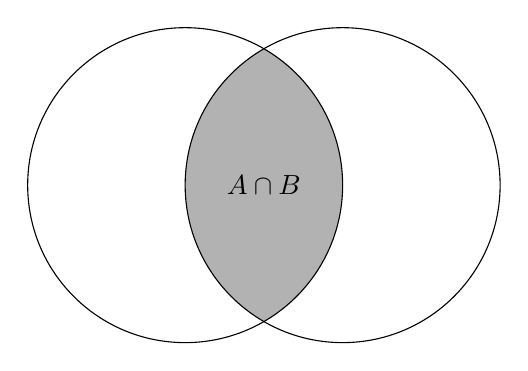
\begin{tikzpicture}
			\path[save path=\pathA](-1,0)circle(2cm);
			\path[save path=\pathB](+1,0)circle(2cm);
			\begin{scope}
				\clip[use path=\pathA];
				\fill[black!30][use path=\pathB];
			\end{scope}
			\draw[use path=\pathA];
			\draw[use path=\pathB];
			\draw(0,0)node{\(A \cap B\)};
		\end{tikzpicture}
		\subcaption{集合的交}
	\end{subfigure}%
	\begin{subfigure}[b]{\subwidth}
		\centering
		\begin{tikzpicture}
			\path[save path=\pathA,name path=A](-1,0)circle(2cm);
			\path[save path=\pathB,name path=B](+1,0)circle(2cm);
			\path[fill=black!30][use path=\pathA+\pathB];
			\draw[name intersections={of=A and B}]
				(intersection-1)arc[start angle=60,end angle=300,radius=2]
				(intersection-2)arc[start angle=-120,end angle=120,radius=2]
				(intersection-1);
			\draw(0,0)node{\(A \cup B\)};
			\pgfresetboundingbox
			\path[use as bounding box] (-3,-2)rectangle(3,2);
		\end{tikzpicture}
		\subcaption{集合的并}
	\end{subfigure}%

	\begin{subfigure}[b]{\linewidth}
		\centering
		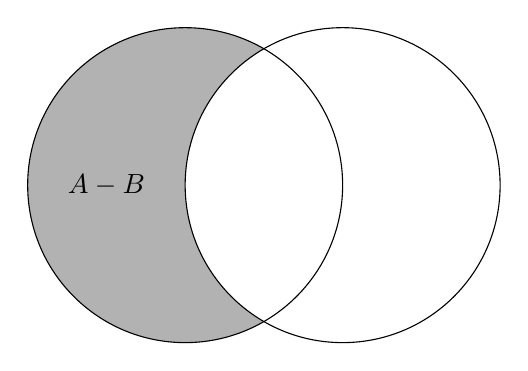
\begin{tikzpicture}
			\fill[black!30](0,{sqrt(3)})arc[start angle=60,end angle=300,radius=2]
				arc[start angle=240,end angle=120,radius=2];
			\draw(-1,0)circle(2cm);
			\draw(+1,0)circle(2cm);
			\draw(-2,0)node{\(A-B\)};
			\pgfresetboundingbox
			\path[use as bounding box] (-3,-2)rectangle(3,2);
		\end{tikzpicture}
		\subcaption{集合的差}
	\end{subfigure}%
	\caption{韦恩图}
	\label{figure:集合论.韦恩图}
\end{figure}

\begin{property}
集合的运算满足以下性质:
\begin{enumerate}
\item 交换律({\rm Commutative laws})
\begin{gather}
A \cap B = B \cap A, \label{equation:集合论.集合代数公式1} \\
A \cup B = B \cup A. \label{equation:集合论.集合代数公式2}
\end{gather}

\item 结合律({\rm Associative laws})
\begin{gather}
(A \cap B) \cap C = A \cap (B \cap C), \label{equation:集合论.集合代数公式3} \\
(A \cup B) \cup C = A \cup (B \cup C). \label{equation:集合论.集合代数公式4}
\end{gather}

\item 分配律({\rm Distributive laws})
\begin{gather}
(A \cap B) \cup C = (A \cup C) \cap (B \cup C), \label{equation:集合论.集合代数公式5} \\
(A \cup B) \cap C = (A \cap C) \cup (B \cap C), \label{equation:集合论.集合代数公式6} \\
A \cup \bigcap \mathscr{B} = \bigcap\Set{A \cup X \given X \in \mathscr{B}}, \quad(\mathscr{B}\neq\emptyset) \label{equation:集合论.集合代数公式5'} \\
A \cap \bigcup \mathscr{B} = \bigcup\Set{A \cap X \given X \in \mathscr{B}}. \label{equation:集合论.集合代数公式6'}
\end{gather}

\item 对偶律({\rm De Morgan's laws})(假设\(\mathscr{A}\neq\emptyset\))
\begin{gather}
\overline{A \cap B} = \overline A \cup \overline B, \label{equation:集合论.集合代数公式7} \\
\overline{A \cup B} = \overline A \cap \overline B, \label{equation:集合论.集合代数公式8} \\
C - \bigcup\mathscr{A} = \bigcap\Set{C-X \given X\in\mathscr{A}}, \label{equation:集合论.集合代数公式7'} \\
C - \bigcap\mathscr{A} = \bigcup\Set{C-X \given X\in\mathscr{A}}. \label{equation:集合论.集合代数公式8'}
\end{gather}

\item 与空集\(\emptyset\)和全集\(\Omega\)的运算(假设\(A \subseteq \Omega\))
\begin{gather}
A \cup \emptyset = A, \label{equation:集合论.集合代数公式9} \\
A \cap \emptyset = \emptyset, \label{equation:集合论.集合代数公式10} \\
A \cup \Omega = \Omega, \label{equation:集合论.集合代数公式11} \\
A \cap \Omega = A, \label{equation:集合论.集合代数公式12} \\
A \cup \overline{A} = \Omega, \label{equation:集合论.集合代数公式13} \\
A \cap \overline{A} = \emptyset. \label{equation:集合论.集合代数公式14}
\end{gather}

\item 包含关系的单调性
\begin{gather}
A \subseteq B \implies A \cup C \subseteq B \cup C, \label{equation:集合论.集合代数公式15} \\
A \subseteq B \implies A \cap C \subseteq B \cap C, \label{equation:集合论.集合代数公式16} \\
A \subseteq B \implies \bigcup A \subseteq \bigcup B, \label{equation:集合论.集合代数公式17} \\
A \subseteq B \implies \overline{B} \subseteq \overline{A}, \label{equation:集合论.集合代数公式18} \\
\emptyset \neq A \subseteq B \implies \bigcap B \subseteq \bigcap A. \label{equation:集合论.集合代数公式19}
\end{gather}
\end{enumerate}
\begin{proof}
对于\cref{equation:集合论.集合代数公式19},假设\(x \in A = \Set{\v{a}{0}} \implies x \in B = \Set{\v{b}{0}}\),%
那么
\begin{align*}
x \in \bigcap B = \bigcap_i b_i
&\iff
	x \in b_i\ (i=1,2,\dotsc) \\
&\implies
	x \in a_i\ (i=1,2,\dotsc) \\
&\iff
	x \in \bigcap_i a_i = \bigcap A.
\qedhere
\end{align*}
\end{proof}
\end{property}

\begin{example}
%@see: 《Elements of Set Theory》 P32. Exercise 21.
设\(A,B\)是集合.
证明:\begin{equation}
	\bigcup(A \cup B) = \bigcup A \cup \bigcup B.
\end{equation}
%TODO
%\begin{proof}
%直接计算得
%\begin{align*}
%	t \in \bigcup(A \cup B)
%	&\iff \exists x \in A \cup B \bigl(
%		t \in x
%	\bigr) \\
%	&\iff \exists x \bigl(
%		x \in A \lor x \in B
%		\implies
%		t \in x
%	\bigr) \\
%	&\iff
%		\exists x \in A \bigl( t \in x \bigr)
%		\lor
%		\exists x \in B \bigl( t \in x \bigr) \\
%	&\iff t \in \bigcup A \lor t \in \bigcup B \\
%	&\iff t \in \bigcup A \cup \bigcup B.
%	\qedhere
%\end{align*}
%\end{proof}
\end{example}

\begin{example}
%@see: 《Elements of Set Theory》 P32. Exercise 22.
设\(A,B\)是非空集合.
证明:\begin{equation}
	\bigcap(A \cup B) = \bigcap A \cap \bigcap B.
\end{equation}
%TODO
%\begin{proof}
%直接计算得\begin{align*}
%	t \in \bigcap(A \cup B)
%	&\iff
%	\forall x \in A \cup B \bigl(
%		t \in x
%	\bigr) \\
%	&\iff
%	\forall x \bigl(
%		x \in A \lor x \in B
%		\implies
%		t \in x
%	\bigr) \\
%	&\iff
%	\forall x \in A \bigl( t \in x \bigr)
%	\land
%	\forall x \in B \bigl( t \in x \bigr) \\
%	&\iff
%	t \in \bigcap A \land t \in \bigcap B \\
%	&\iff
%	t \in \bigcap A \cap \bigcap B.
%	\qedhere
%\end{align*}
%\end{proof}
\end{example}

\begin{example}
证明:\begin{equation}
	(A \cup B) - (A \cap B) = (A-B)\cup(B-A).
\end{equation}
\begin{proof}
根据集合交、并、差的定义,有
\begin{align*}
	x \in (A \cup B) - (A \cap B)
	&\iff x \in (A \cup B) \land x \notin (A \cap B) \\
	&\iff (x \in A \lor x \in B) \land \neg(x \in A \land x \in B) \\
	&\iff (x \in A \land \neg(x \in A \land x \in B))
	 \lor (x \in B \land \neg(x \in A \land x \in B)) \\
	&\iff (x \in A \land (x \notin A \lor x \notin B))
	 \lor (x \in B \land (x \notin A \lor x \notin B)) \\
	&\iff (x \in A \land x \notin B) \lor (x \in B \land x \notin A) \\
	&\iff x \in (A-B)\cup(B-A).
\qedhere
\end{align*}
\end{proof}
\end{example}

\section{关系}
\subsection{无序对、有序对的概念}
\begin{definition}[无序对]
由两个元素\(x_1\)和\(x_2\)组成的集合\[
\Set{x_1, x_2}
\]称作\DefineConcept{无序对}(unordered pair).
\end{definition}

\begin{example}
%@see: 《Elements of Set Theory》 P38. Exercise 1.
定义:\[
\opair{x,y,z}^* = \{\{x\},\{x,y\},\{x,y,z\}\}.
\]找出元素\(u,v,w,x,y,z\)使\[
\opair{x,y,z}^* = \opair{u,v,w}^*
\]成立,但\(y \neq v\)或\(z \neq w\).
\begin{solution}
取\[
\opair{1,1,2}^* = \{\{1\},\{1,1\},\{1,1,2\}\} = \{\{1\},\{1,2\}\},
\]\[
\opair{1,2,1}^* = \{\{1\},\{1,2\},\{1,2,1\}\} = \{\{1\},\{1,2\}\},
\]即可满足题设条件.
\end{solution}
\end{example}

\begin{definition}[有序对]
两个元素\(x_1\)和\(x_2\)按一定顺序形成的排列称为\DefineConcept{有序对},记作\[
\opair{x_1,x_2}.
\]

我们可以采用多种方式构造集合用于表记有序对\(\opair{x_1,x_2}\),例如(由Norbert Wiener于1914年构造的)
\[
\Set{ \Set{ \Set{x_1}, \emptyset }, \Set{ \Set{ x_2 } } }.
\]
但我们更常用(由Kazimierz Kuratowski于1921年构造的)以下形式
\[
\Set{ \Set{x_1}, \Set{x_1, x_2} }.
\]以后我们都采用第二种形式表记有序对,因此\[
\opair{x_1,x_2}
\defeq
\Set{ \Set{x_1}, \Set{x_1, x_2} }.
\]
\end{definition}

有序对具有以下性质.
\begin{property}\label{theorem:集合论.有序对的性质1}
%@see: 《Elements of Set Theory》 P36. Theorem 3A
\(\opair{u,v} = \opair{x,y}\)的充要条件是:\(u=x\)且\(v=y\).
\begin{proof}
充分性.
这个方向的证明是平凡的;
当\(u=x\)且\(v=y\)时,自然有\[
	\opair{u,v} = \opair{x,y}.
\]

必要性.
当\(\opair{u,v} = \opair{x,y}\)时,根据定义有\[
	\Set{ \Set{u}, \Set{u, v} }
	= \Set{ \Set{x}, \Set{x, y} };
\]于是\[
	\Set{u} \in \Set{ \Set{x}, \Set{x, y} },
	\eqno{(1)}
\]且\[
	\Set{u,v} \in \Set{ \Set{x}, \Set{x, y} }.
	\eqno{(2)}
\]
从(1)式我们知道,要么等式\[
	\Set{u} = \Set{x}
	\eqno{(3)}
\]成立,要么等式\[
	\Set{u} = \Set{x,y}
	\eqno{(4)}
\]成立;
从(2)式我们知道,要么等式\[
	\Set{u,v} = \Set{x}
	\eqno{(5)}
\]成立,要么等式\[
	\Set{u,v} = \Set{x,y}
	\eqno{(6)}
\]成立.

首先我们假设(4)式成立,那么有\(u = x = y\);
从而有(5)式等价于(6)式,且\(u = v = x = y\);
在这种情况下,必要性得证.
同理,假设(5)式成立,也可证明必要性.

然后我们假设(3)式、(6)式同时成立.
从(3)式成立我们知道\(u = x\).
从(6)式成立我们知道\(u = y\)或\(v = y\);
第一种情况,即\(u = x\)和\(u = y\)同时成立的情况,已经在(4)式成立时作了讨论.
第二种情况,即\(u = x\)和\(v = y\)同时成立的情况,立即保证了必要性.
\end{proof}
\end{property}
\cref{theorem:集合论.有序对的性质1} 让我们可以不含糊地将有序对\(\opair{x,y}\)
中的\(x\)和\(y\)分别称为%
有序对的\DefineConcept{第一坐标}(first coordinate)%
和\DefineConcept{第二坐标}(second coordinate).

\subsection{直积}
\begin{definition}[直积]\label{definition:集合论.直积}
设\(A,B\)都是集合.
在\(A\)中任取一个元素\(x\),
在\(B\)中任取一个元素\(y\),
组成一个有序对\(\opair{x,y}\),
把这样的有序对作为新的元素,
它们全体组成的集合称为“\(A\)与\(B\)的%
\DefineConcept{直积}或\DefineConcept{笛卡尔乘积}(Cartesian product)”,
记为\(A \times B\),即\[
	A \times B
	\defeq
	\Set{ \opair{x,y} \given x \in A, y \in B }.
\]

特别地,集合\(A\)与自己的直积\(A \times A\)可以简记为\(A^2\),
\((A \times A) \times A\)可以简记为\(A^3\),以此类推.
\end{definition}

在宣称\cref{definition:集合论.直积} 合法以前,
我们必须确认它给出的收集\(A \times B\)是不是真的是一个集合.
设符号\(\lambda(t)\)表示“与\(t\)有关的命题公式”,
我们在运用描述法记号\[
	\Set{ t \given \lambda(t) }
\]表记一个集合时,必须验证是不是真的存在一个集合\(D\),使得\[
	\forall t \bigl( t \in D \iff \lambda(t) \bigr)
\]成立.
例如,虽然\[
	\Set{ x \given x = x }
	\quad\text{和}\quad
	\Set{ x \given x \neq x }
\]这两个表达式看起来相似,
但根据\cref{theorem:集合论.以所有集合为元素组成的集合不存在},
这里的第一个表达式不能表示一个集合;
然而根据空集公理,第二个表达式就可以表示空集.

要证明\(A \times B\)是一个集合,
我们就必须找到一个足够大的集合,
它包括了我们需要的全部有序对,
然后利用子集公理证明\(A \times B\)是这个集合的子集.
因此,我们给出下述引理.
\begin{lemma}\label{theorem:集合论.有序对是其坐标元素所在集合的二重幂集的元素}
%@see: 《Elements of Set Theory》 P37. Lemma 3B
如果\(x,y \in A\),那么\[
	\opair{x,y} \in \Powerset\Powerset A.
\]
\begin{proof}
由\(x,y \in A\)可知\(\{x\},\{x,y\} \subseteq A\),
即\(\{x\},\{x,y\} \in \Powerset A\),
那么\(\{\{x\},\{x,y\}\} \subseteq \Powerset A\),
进一步可得\(\{\{x\},\{x,y\}\} \in \Powerset\Powerset A\).
\end{proof}
\end{lemma}

\begin{theorem}\label{theorem:集合论.直积存在定理}
%@see: 《Elements of Set Theory》 P38. Corollary 3C
对任意集合\(A,B\),存在这样一个集合,
它的元素全是有序对\(\opair{x,y}\),
其中\(x \in A\),\(y \in B\).
\begin{proof}
根据子集公理,我们可以构造集合\[
	\Set*{ w \in \Powerset\Powerset(A \cup B) \given w = \opair{x,y}, x \in A, y \in B }.
\]
显然,根据\cref{theorem:集合论.有序对是其坐标元素所在集合的二重幂集的元素},
这个集合仅包括我们需要的有序对.
\end{proof}
\end{theorem}
依靠\cref{theorem:集合论.直积存在定理},
我们就可以正当化先前对\hyperref[definition:集合论.直积]{直积}\(A \times B\)的定义.

容易发现,对于任意集合\(A\),总有\begin{equation}
	A \times \emptyset
	= \emptyset \times A
	= \emptyset \times \emptyset
	= \emptyset.
\end{equation}

\begin{example}
%@see: 《Elements of Set Theory》 P38. Exercise 2.(a)
%@see: 《Elements of Set Theory》 P65. Exercise 54.
设\(A,B,C\)是集合.
证明:\begin{gather}
	A \times (B \cup C) = (A \times B) \cup (A \times C),
	\label{equation:集合论.直积分配律1} \\
	A \times (B \cap C) = (A \times B) \cap (A \times C),
	\label{equation:集合论.直积分配律2} \\
	A \times (B - C) = (A \times B) - (A \times C).
	\label{equation:集合论.直积分配律3}
\end{gather}
\begin{proof}
对\cref{equation:集合论.直积分配律1} 证明如下:
由于对于任意\(w = \opair{x,y}\)总有
\begin{align*}
	w \in A \times (B \cup C)
	&\iff x \in A \land y \in B \cup C \\
	&\iff x \in A \land (y \in B \lor y \in C) \\
	&\iff (x \in A \land y \in B) \lor (x \in A \land y \in C) \\
	&\iff (w \in A \times B) \lor (w \in A \times C),
\end{align*}
那么由外延公理可知\(A \times (B \cup C) = (A \times B) \cup (A \times C)\).

对\cref{equation:集合论.直积分配律2} 证明如下:
由于对于任意\(w = \opair{x,y}\)总有
\begin{align*}
	w \in A \times (B \cap C)
	&\iff x \in A \land y \in B \cap C \\
	&\iff x \in A \land (y \in B \land y \in C) \\
	&\iff (x \in A \land y \in B) \land (x \in A \land y \in C) \\
	&\iff (w \in A \times B) \land (w \in A \times C),
\end{align*}
那么由外延公理可知\(A \times (B \cap C) = (A \times B) \cap (A \times C)\).

对\cref{equation:集合论.直积分配律3} 证明如下:
由于对于任意\(w = \opair{x,y}\)总有
\begin{align*}
	w \in A \times (B - C)
	&\iff x \in A \land y \in (B - C) \\
	&\iff x \in A \land (y \in B \land y \notin C) \\
	&\iff (x \in A \land y \in B \land x \notin A)
		\lor (x \in A \land y \in B \land y \notin C) \\
	&\iff (x \in A \land y \in B) \land (x \notin A \lor y \notin C) \\
	&\iff (x \in A \land y \in B) \land \neg(x \in A \land y \in C) \\
	&\iff w \in A \times B \land w \notin A \times C,
\end{align*}
那么由外延公理可知\(A \times (B - C) = (A \times B) - (A \times C)\).
\end{proof}
\end{example}

\begin{example}
%@see: 《Elements of Set Theory》 P38. Exercise 2.(b)
证明:如果\(A \times B = A \times C\)且\(A \neq \emptyset\),则\(B = C\).
%TODO
\end{example}

\begin{example}
%@see: 《Elements of Set Theory》 P38. Exercise 3.
证明:\(A \times \bigcup B = \bigcup\Set{ A \times X \given X \in B }\).
%TODO
\end{example}

\begin{example}
%@see: 《Elements of Set Theory》 P38. Exercise 5.(a)
设\(A,B\)都是集合,试证:\(\Set{ \{x\} \times B \given x \in A }\)也是集合.
%TODO
\end{example}

\subsection{关系}
\begin{definition}
\DefineConcept{关系}(relation)是有序对的集合.
\end{definition}

如果有序对\(\opair{x,y}\)是关系\(\rel{R}\)的元素,即\[
	\opair{x,y} \in \rel{R},
\]
那么称“\(x\)与\(y\)有\(\rel{R}\)关系”,
记作\(x\rel{R}y\);
反之,\[
	\opair{x,y} \notin \rel{R},
\]
那么称“\(x\)与\(y\)没有\(\rel{R}\)关系”.

给定集合\(X\)和集合\(Y\),
如果关系\(\rel{R}\)满足\[
	\rel{R} \subseteq X \times Y,
\]
我们就称“\(\rel{R}\)是\(X\)与\(Y\)之间的\DefineConcept{二元关系}(binary relation)”.
特别地,当\(X = Y\)时,就称“\(\rel{R}\)是\(X\)上的\DefineConcept{二元关系}”.

从关系的定义可以看出,关系是有序对的集合.
即便是看起来毫无意义的,只由一个有序对组成的集合,也可以看成是一个关系.
我们自然会认为有的关系比别的关系更有意义,
例如我们马上会提到的“映射”“等价关系”和“排序关系”.

\begin{definition}\label{definition:集合论.定义域与值域的定义}
设\(R\)是集合.

如果集合\(A\)满足\[
	x \in A \iff \exists y \bigl( \opair{x,y} \in R \bigr),
\]
那么称\(A\)为“\(R\)的\DefineConcept{定义域}(domain)”,记作\(\dom R\).

如果集合\(B\)满足\[
	x \in B \iff \exists t \bigl( \opair{t,x} \in R \bigr),
\]
那么称\(B\)为“\(R\)的\DefineConcept{值域}(range)”,记作\(\ran R\).

最后,我们把\(R\)的定义域与它的值域的并集称为
“\(R\)的\DefineConcept{域}(field)”,记作\(\fld R\),即\[
	\fld R \defeq \dom R \cup \ran R.
\]
\end{definition}

为了正当化\cref{definition:集合论.定义域与值域的定义},
我们必须明确:对于任意集合\(R\),存在这样一个集合,
\(R\)中的有序对的第一坐标和第二坐标都是这个集合的元素.
这个问题类似于我们之前对于直积\(A \times B\)的定义的正当化,
当时我们证明了\cref{theorem:集合论.直积存在定理}.
为此,我们给出下述引理,
可以注意到它与\cref{theorem:集合论.有序对是其坐标元素所在集合的二重幂集的元素} 的关联.

\begin{lemma}
%@see: 《Elements of Set Theory》 P38. Lemma 3D
如果\(\opair{x,y} \in A\),那么\(x,y \in \bigcup\bigcup A\).
\end{lemma}
这条引理已经在\cref{example:集合论.有序对各坐标的取值范围} 得到证明.
利用这条引理,再加上子集公理,我们可以构造集合\(R\)的定义域和值域:
\begin{gather}
	\dom R
	\defeq
	\Set*{ x \in \bigcup\bigcup R \given \exists y \bigl( \opair{x,y} \in R \bigr) }, \\
	\ran R
	\defeq
	\Set*{ x \in \bigcup\bigcup R \given \exists t \bigl( \opair{t,x} \in R \bigr) }.
\end{gather}

\begin{example}
%@see: 《Elements of Set Theory》 P41. Exercise 6.
试证:集合\(A\)是一个关系的充要条件是\[
	A \subseteq \dom A \times \ran A.
\]
%TODO
\end{example}

\begin{example}
%@see: 《Elements of Set Theory》 P41. Exercise 7.
试证:给定关系\(\rel{R}\),总有\[
	\fld \rel{R} = \bigcup\bigcup \rel{R}.
\]
%TODO
\end{example}

\begin{example}
%@see: 《Elements of Set Theory》 P41. Exercise 8.
试证:对于任意集合\(A\),总有\begin{gather}
	\dom\bigcup A = \bigcup\Set{ \dom\rel{R} \given \rel{R} \in A }, \\
	\ran\bigcup A = \bigcup\Set{ \ran\rel{R} \given \rel{R} \in A }.
\end{gather}
%TODO
\end{example}

\subsection{多元关系}
我们可以将“有序对”和“二元关系”的概念分别扩展为“元组”和“多元关系”.

例如定义\[
	\opair{x_1,x_2,x_3}
	\defeq
	\opair{\opair{x_1,x_2},x_3},
\]
称之为\DefineConcept{三元组}(triple);
定义\[
	\opair{x_1,x_2,x_3,x_4}
	\defeq
	\opair{\opair{x_1,x_2,x_3},x_4},
\]
称之为\DefineConcept{四元组}(quadruple);
定义\[
	\opair{x_1,x_2,x_3,x_4,x_5}
	\defeq
	\opair{\opair{x_1,x_2,x_3,x_4},x_5},
\]
称之为\DefineConcept{五元组}(quintuple);
以此类推,对于任意给定\(n\),可以定义\(n\)元组(\(n\)-tuple):\[
	\opair{x_1,x_2,\dotsc,x_n}
	\defeq
	\opair{\opair{x_1,x_2,\dotsc,x_{n-1}},x_n}.
\]
为了让我们的定义看起来整齐划一,我们还可以补充定义\[
	\opair{x} \defeq x,
\]
称之为\DefineConcept{一元组}(1-tuple).

我们把“在\(A\)上的\(n\)元\DefineConcept{关系}(n-ary \emph{relation} on \(A\))”%
定义为由\(n\)元组构成的集合.
由于\(A\)上的二元关系是\(A \times A\)的子集,
以及\(A\)上的三元关系(ternary relation, 3-ary relation)是\((A \times A) \times A\)的子集,
所以三元关系也可归结为一种二元关系;
同理,其他\(n\)元关系,只要\(n>1\),也都可以归结为二元关系.
虽然在上面对\(n\)元关系的定义中,
我们也把由\(A\)中包括的一元组构成的集合称为%
“\(A\)上的一元关系(unary relation, 1-ary relation)”,
但它只是\(A\)的一个子集,根本不满足关系的定义.

\section{映射}
\subsection{映射的概念}
\begin{definition}
设\(F\)是关系,如果\[
	\forall x \in \dom F, \exists! y:
	x F y,
\]
则称“关系\(F\)是一个\DefineConcept{映射}(function)”.
\end{definition}
可以从映射的定义中看出,虽然映射也是关系,
但映射有一般的关系所没有的特殊性质:
映射是\DefineConcept{单值的}(single-valued).
换句话说,对于关系\(F\),每个\(x\)可能对应若干个\(y\);
但是,对于映射\(F\),每个\(x\)就只对应一个\(y\).
我们可以把\(x\)与\(y\)这两个元素之间的对应关系记为\(x \mapsto y\).

我们把使得\(xFy\)成立的\(y\)称为“\(x\)(在映射\(F\)下)的\DefineConcept{像}%
(the \emph{value} of \(F\) at \(x\))”,
记为\(F(x)\),即\[
	y = f(x);
\]
称\(x\)为“\(y\)(在映射\(F\)下)的一个\DefineConcept{原像}”.
这里用的\(F(x)\)符号是欧拉提出的,
我们仅当\(F\)是一个映射且\(x\in\dom F\)时使用这个记号.
不过,我们也可以定义:\[
	F(x) \defeq \bigcup\Set{ y \given \opair{x,y} \in F }.
\]
它对于任意\(F\)和\(x\)都有意义.

映射是如此重要,以至于各家对用于描述映射的术语没有达成统一.
以下是两种最常采用的术语.

设\(X,Y\)都是集合,
如果\(f\)是一个映射,且\(\dom f = X\),\(\ran f \subseteq Y\),
则称“\(f\)是从\(X\)到\(Y\)的\DefineConcept{映射}%
(\(f\) is a function \emph{from} \(X\) \emph{into} \(Y\))”,
或称“\(f\)将\(X\)映射到\(Y\)里%
(\(f\) \emph{maps} \(X\) \emph{into} \(Y\))”,
记作\[
	f\colon X \to Y.
\]
如果还有\(\ran f = Y\),
那么称“\(f\)是从\(X\)到\(Y\)上的映射%
(\(f\) is a function from \(X\) \emph{onto} \(Y\))”,
或称“\(f\)将\(X\)映射到\(Y\)上%
(\(f\) \emph{maps} \(X\) \emph{onto} \(Y\))”,
或称“\(f\)是\DefineConcept{满射}(surjective)”.
我们可以说“任意映射总将它的定义域映射到它的值域上”,
还可以说“任意映射总把它的定义域映射到以它的值域为子集的任意集合\(B\)里”.
注意到两种说法的区别,“上”字和“里”字的选用,
不光取决于映射\(f\)本身,还取决于我们讨论的集合\(B\).

如果\[
	\forall y \in \ran f,
	\exists! x \bigl( x f y \bigr),
\]
那么称“映射\(f\)是\DefineConcept{一一映射}(one-to-one)”.

有时候我们希望把一一映射的概念套用到一般的关系上,
它们往往不是映射,因此“一一映射”这个用词就显得不那么恰当了.
为此,我们创造出“单根的”,类比于“单值的”.

\begin{definition}
如果集合\(R\)满足\[
	\forall y \in \ran R,
	\exists! x:
	x R y,
\]
则称“\(R\)是\DefineConcept{单根的}(single-rooted)”.
\end{definition}

因此,我们可以说,“一个映射是单根的”当且仅当“这个映射是一一映射”.

如果\[
	\forall x_1, x_2 \in \dom f
	\bigl[ x_1 \neq x_2 \implies f(x_1) \neq f(x_2) \bigr],
\]
那么称“\(f\)是\DefineConcept{单射}(injective)”.
由于映射本就是单值的,若它还是单根的,那么这个映射就是单射;
换句话说,一一映射和单射是相同的概念.

如果\(f\)既是单射,又是满射,即
那么称“\(f\)是\DefineConcept{双射}(bijective)\footnote{%
有的书可能会把双射称作一一映射,但是我们不采取这种说法.
}”.


\begin{example}
设\(f\colon A \to B, g\colon B \to C\).
证明:\begin{enumerate}
	\item 如果\(f\)和\(g\)都是单射,那么\(g \circ f\)也是单射;
	\item 如果\(f\)和\(g\)都是满射,那么\(g \circ f\)也是满射;
	\item 如果\(f\)和\(g\)都是双射,那么\(g \circ f\)也是双射;
	\item 如果\(f\)和\(g\)都是可逆映射,那么\(g \circ f\)也是可逆映射.
\end{enumerate}
\begin{proof}
当\(f\)和\(g\)都是单射时.设\(a_1,a_2 \in A\).
如果\((g \circ f)(a_1) = (g \circ f)(a_2)\),那么\(g[f(a_1)] = g[f(a_2)]\).
由于\(g\)是单射,因此\(f(a_1) = f(a_2)\).
由于\(f\)是单射,因此\(a_1 = a_2\).
综上,\(g \circ f\)是单射.

当\(f\)和\(g\)都是满射时.任取\(c \in C\).
由于\(g\)是满射,因此存在\(b \in B\),使得\(c = g(b)\).
由于\(f\)是满射,因此存在\(a \in A\),使得\(b = f(a)\).
因此\(c = g(b) = g[f(a)] = (g \circ f)(a)\),也就是说\(g \circ f\)是满射.

双射的情形,根据单射、满射的情形显然成立.

可逆映射的情形,根据双射的情形以及\cref{theorem:集合论.映射可逆的充要条件} 即得.
\end{proof}
\end{example}


\subsection{逆,复合,限制,像,原像}
以下定义的操作通常用在映射上,有时候也用于关系,但也可以用于任意集合.
\begin{definition}
设\(A,F,G\)都是集合.
\begin{enumerate}
	\item 称集合\[
		\Set*{ \opair{u,v} \given v F u }
	\]为“\(F\)的\DefineConcept{逆}%
	(the \emph{inverse} of \(F\))”,
	记作\(F^{-1}\).

	特别地,如果\(F^{-1}\)是映射,
	则称“\(F^{-1}\)是\(F\)的\DefineConcept{逆映射}”.

	\item 称集合\[
		\Set*{ \opair{u,v} \given \exists t \bigl( u G t \land t F v \bigr) }
	\]为“\(F\)和\(G\)的\DefineConcept{复合}%
	(the \emph{composition} of \(F\) and \(G\))”,
	记作\(F \circ G\).

	\item 称集合\[
		\Set*{ \opair{u,v} \given u F v \land u \in A }
	\]为“\(F\)在\(A\)上的\DefineConcept{限制}%
	(the \emph{restriction} of \(F\) to \(A\))”,
	记作\(F \upharpoonright A\).

	\item 称集合\[
		\Set*{ v \given \exists u \in A \bigl( u F v \bigr) }
	\]为“\(A\)在\(F\)下的\DefineConcept{像}%
	(the \emph{image} of \(A\) \emph{under} \(F\))”,
	记作\(F\ImageOfSetUnderRelation{A}\).
\end{enumerate}
\end{definition}

当\(F\)是一个映射,且\(A \subseteq \dom F\)时,
\(F\ImageOfSetUnderRelation{A}\)这个概念可能更容易理解,
因为这时候\[
	F\ImageOfSetUnderRelation{A}
	= \Set{ F(u) \given u \in A }.
\]

我们可以利用子集公理构造出上述定义下的所需集合的存在性.
特别地,\[
	F^{-1} \subseteq \ran F \times \dom F, \qquad
	F \circ G \subseteq \dom G \times \ran F,
\]\[
	F \upharpoonright A \subseteq F, \qquad
	F\ImageOfSetUnderRelation{A} \subseteq \ran F.
\]

例如,我们可以按如下方法正当化“关系\(F\)的逆”的定义:
根据子集公理,存在集合\(B\),使得对于任意\(x\),总有\begin{align*}
	x \in B
	&\iff
	x \in \ran F \times \dom F
	\land
	\exists u, \exists v \bigl( x = \opair{u,v} \land v F u \bigr), \\
	&\iff
	\exists u, \exists v \bigl( x = \opair{u,v} \land v F u \bigr).
\end{align*}
再根据外延公理,可以保证集合\(B\)的唯一性.
因此我们可以将集合\(B\)记为\(F^{-1}\).

\begin{theorem}
\(F \upharpoonright \emptyset = \emptyset\).
\end{theorem}

\begin{theorem}
\(F\ImageOfSetUnderRelation{A} = \ran(F \upharpoonright A)\).
\begin{proof}
根据值域的定义有\begin{align*}
	v \in \ran(F \upharpoonright A)
	&\iff
	\exists u \bigl( \opair{u,v} \in F \upharpoonright A \bigr) \\
	&\iff
	\exists u \bigl( u F v \land u \in A \bigr) \\
	&\iff
	v \in F\ImageOfSetUnderRelation{A}.
	\qedhere
\end{align*}
\end{proof}
\end{theorem}

\begin{definition}
设\(F\)是关系,\(A\)是集合,那么称集合\[
	\Set*{ x \in \dom F \given F(x) \in A }
\]为“集合\(A\)在关系\(F\)下的\DefineConcept{原像}%
(the \emph{inverse image} of \(A\) under \(F\))”,
记作\(F^{-1}\ImageOfSetUnderRelation{A}\).
\end{definition}

\begin{theorem}\label{theorem:集合论.关系的逆的定义域值域以及关系的二重逆}
%@see: 《Elements of Set Theory》 P46. Theorem 3E
设\(F\)是集合,则有\begin{gather}
	\dom F^{-1} = \ran F, \\
	\ran F^{-1} = \dom F.
\end{gather}

如果\(F\)是关系,则有\begin{equation}
	(F^{-1})^{-1} = F.
\end{equation}
\end{theorem}

\begin{theorem}\label{theorem:集合论.关系及其逆是映射的充要条件}
%@see: 《Elements of Set Theory》 P46. Theorem 3F
设\(F\)是集合,则“\(F^{-1}\)是映射”的充要条件是:\(F\)是单根的.

设\(F\)是关系,则“\(F\)是映射”的充要条件是:\(F^{-1}\)是单根的.
\end{theorem}

\begin{theorem}\label{theorem:集合论.映射可逆的充要条件}
映射\(f\)可逆的充要条件是:\(f\)是双射.
\end{theorem}

\begin{theorem}
%@see: 《Elements of Set Theory》 P46. Theorem 3G
设\(F\)是一一映射.
\begin{enumerate}
	\item 如果\(x \in \dom F\),那么\[
		F^{-1}(F(x)) = x.
	\]

	\item 如果\(y \in \ran F\),那么\[
		F(F^{-1}(y)) = y.
	\]
\end{enumerate}
\begin{proof}
假设\(x \in \dom F\),
那么\(\opair{x,F(x)} \in F\),且\(\opair{F(x),x} \in F^{-1}\),
于是\(F(x) \in \dom F^{-1}\).
因为\(F\)是一一映射,是单值的,所以\(F^{-1}\)是映射,
从而\(x = F^{-1}(F(x))\).

如果\(y \in \ran F\),
那么根据本定理第1条,以及\((F^{-1})^{-1} = F\),可知\[
	F(F^{-1}(y)) = (F^{-1})^{-1}(F^{-1}(y)) = y.
	\qedhere
\]
\end{proof}
\end{theorem}

\begin{theorem}
%@see: 《Elements of Set Theory》 P47. Theorem 3H
设\(F,G\)都是映射,则\(F \circ G\)是映射,且\[
	\dom(F \circ G)
	= \Set*{ x \in \dom G \given G(x) \in \dom F },
\]\[
	\forall x \in \dom(F \circ G):
	(F \circ G)(x) = F(G(x)).
\]
\begin{proof}
要证\(F \circ G\)是一个映射,
假设有\(x (F \circ G) y\)和\(x (F \circ G) z\)同时成立.
那么,\(\exists p,q\),有\[
	x G p \land p F y
	\quad\text{和}\quad
	x G q \land q F z
\]同时成立.
既然\(G\)是映射,必有\(p = q\).
同理,\(F\)是映射,必有\(y = z\).
因此\(F \circ G\)是映射.

现在再假设\(x \in \dom G\)且\(G(x) \in \dom F\).
我们必须证明\[
	x \in \dom(F \circ G)
	\quad\text{和}\quad
	(F \circ G)(x) = F(G(x)).
\]
我们知道\[
	\opair{x,G(x)} \in G,
	\qquad
	\opair{G(x),F(G(x))} \in F.
\]
因此\(\opair{x,F(G(x))} \in F \circ G\).

反过来说,如果\(x \in \dom(F \circ G)\),
那么就有\[
	\exists y, \exists t
	\bigl( x G t \land t F y \bigr).
\]
于是就有\(x \in \dom G\)和\(t = G(x) \in \dom F\).
\end{proof}
\end{theorem}

容易看出,映射的复合是有顺序的,\(f \circ g\)有意义并不代表\(g \circ f\)也有意义.
即便两者都有意义,它们也未必相同.

\begin{theorem}
%@see: 《Elements of Set Theory》 P65. Exercise 53.
设\(R,S\)是集合,那么\begin{gather}
	(R \cup S)^{-1} = R^{-1} \cup S^{-1},
	\label{equation:集合论.并的逆等于逆的并} \\
	(R \cap S)^{-1} = R^{-1} \cap S^{-1},
	\label{equation:集合论.交的逆等于逆的交} \\
	(R - S)^{-1} = R^{-1} - S^{-1}.
	\label{equation:集合论.差的逆等于逆的差}
\end{gather}
\begin{proof}
对\cref{equation:集合论.并的逆等于逆的并} 证明如下:
\begin{align*}
	\opair{x,y} \in (R \cup S)^{-1}
	&\iff \opair{y,x} \in R \cup S \\
	&\iff \opair{y,x} \in R \lor \opair{y,x} \in S \\
	&\iff \opair{x,y} \in R^{-1} \lor \opair{x,y} \in S^{-1} \\
	&\iff \opair{x,y} \in R^{-1} \cup S^{-1}.
\end{align*}

对\cref{equation:集合论.交的逆等于逆的交} 证明如下:
\begin{align*}
	\opair{x,y} \in (R \cap S)^{-1}
	&\iff \opair{y,x} \in R \cap S \\
	&\iff \opair{y,x} \in R \land \opair{y,x} \in S \\
	&\iff \opair{x,y} \in R^{-1} \land \opair{x,y} \in S^{-1} \\
	&\iff \opair{x,y} \in R^{-1} \cap S^{-1}.
\end{align*}

对\cref{equation:集合论.差的逆等于逆的差} 证明如下:
\begin{align*}
	\opair{x,y} \in (R - S)^{-1}
	&\iff \opair{y,x} \in R - S \\
	&\iff \opair{y,x} \in R \land \opair{y,x} \notin S \\
	&\iff \opair{x,y} \in R^{-1} \land \opair{x,y} \notin S^{-1} \\
	&\iff \opair{x,y} \in R^{-1} - S^{-1}.
	\qedhere
\end{align*}
\end{proof}
\end{theorem}

\begin{theorem}
%@see: 《Elements of Set Theory》 P47. Theorem 3I
设\(F,G\)都是集合,那么\[
	(F \circ G)^{-1} = G^{-1} \circ F^{-1}.
\]
\begin{proof}
易知\((F \circ G)^{-1}\)和\(G^{-1} \circ F^{-1}\)都是关系,且\begin{align*}
	\opair{x,y} \in (F \circ G)^{-1}
	&\iff
	\opair{y,x} \in F \circ G \\
	&\iff
	\exists t \bigl( y G t \land t F x \bigr) \\
	&\iff
	\exists t \bigl( x F^{-1} t \land t G^{-1} y \bigr) \\
	&\iff
	\opair{x,y} \in G^{-1} \circ F^{-1}.
	\qedhere
\end{align*}
\end{proof}
\end{theorem}

\begin{axiom}[选择公理(第一种形式)]
对于任意关系\(R\),存在映射\(H\),满足\[
	H \subseteq R,
	\quad\text{且}\quad
	\dom H = \dom R.
\]
\end{axiom}

\begin{theorem}
%@see: 《Elements of Set Theory》 P48. Theorem 3J
设映射\(F\colon A \to B\),其中\(A\)是非空集合.
\begin{enumerate}
	\item “存在映射\(G\colon B \to A\)(称其为\DefineConcept{左逆}),
	使得\(G \circ F\)是\(A\)上的恒等映射\(I_A\)”是“\(F\)是一一映射”的充要条件.

	\item “存在映射\(H\colon B \to A\)(称其为\DefineConcept{右逆}),
	使得\(F \circ H\)是\(B\)上的恒等映射\(I_B\)”是“\(F\)是满射”的充要条件.
\end{enumerate}
\begin{proof}
\begin{enumerate}
	\item
	先证充分性.
	我们假设存在映射\(G\)使得\(G \circ F = I_A\).
	如果\(F(x) = F(y)\),那么\[
		x = G(F(x)) = G(F(y)) = y,
	\]
	于是\(F\)是一一映射.

	再证必要性.
	假设\(F\)是一一映射,
	那么根据\cref{theorem:集合论.关系的逆的定义域值域以及关系的二重逆,theorem:集合论.关系及其逆是映射的充要条件},
	\(F^{-1}\)是一个从\(\ran F\)到\(A\)上的映射.
	现在我们需要将\(F^{-1}\)延拓为以\(B\)为定义域的映射\(G\).
	因为\(A\)是非空集合,
	于是我们可以取定\(a \in A\),
	然后令\[
		G(x) = \left\{ \begin{array}{ll}
			F^{-1}(x), & x \in \ran F, \\
			a, & x \in B - \ran F,
		\end{array} \right.
	\]或者令\[
		G = F^{-1} \cup (B - \ran F) \times \Set{a}.
	\]
	这个构造出来的映射\(G\)是一个从\(B\)到\(A\)里的映射,
	且满足\[
		\dom(G \circ F) = A,
	\]
	以及\[
		\forall x \in A: G(F(x)) = F^{-1}(F(x)) = x,
	\]
	于是\(G \circ F = I_A\)成立.

	\item
	我们还是先证充分性.
	假设存在映射\(H\)使得\(F \circ H = I_B\).
	那么\[
		\forall y \in B: y = F(H(y)),
	\]
	从而\(y \in \ran F\),
	于是\(\ran F = B\).

	必要性的证明稍显困难.
	我们不能直接取\(H = F^{-1}\),
	因为一般而言\(F\)不会是一一映射,
	\(F^{-1}\)也不会是一个映射.
	假设\(F\)将\(A\)映射到\(B\)上,\(\ran F = B\).
	现在我们需要为每个\(y \in B\)选择某个\(x\),使得\(F(x) = y\),然后令\(H(y) = x\);
	考虑到\(y \in \ran F\),这样的\(x\)必定存在.
	虽然我们知道对于每个\(y\),存在一个合适的\(x\),
	但是我们无法据此构造所求映射\(H\).
	因此,我们需要引入选择公理.
	借助选择公理,我们可以令映射\(H\)满足\(H \subseteq F^{-1}\)且\(\dom H = \dom F^{-1} = B\).
	于是\(H\)满足\[
		\forall y \in B
		\bigl[
		\opair{y,H(y)} \in F^{-1}
		\iff \opair{H(y),y} \in F
		\iff F(H(y)) = y
		\bigr].
		\qedhere
	\]
\end{enumerate}
\end{proof}
\end{theorem}

\begin{theorem}
%@see: 《Elements of Set Theory》 P48. Theorem 3K
设\(A,B,F\)都是集合.
\def\F#1{F\ImageOfSetUnderRelation{#1}}
\begin{enumerate}
	\item 并的像是像的并:\begin{gather}
		\F{A \cup B}
		= \F{A} \cup \F{B},
		\label{equation:集合论.并的像与像的并的关系1} \\
		\F{\bigcup A}
		= \bigcup\Set{ \F{a} \given a \in A }.
		\label{equation:集合论.并的像与像的并的关系2}
	\end{gather}

	\item 交的像包含于像的交:\begin{gather}
		\F{A \cap B}
		\subseteq \F{A} \cap \F{B},
		\label{equation:集合论.交的像与像的交的关系1} \\
		\F{\bigcap A}
		\subseteq \bigcap\Set{ \F{a} \given a \in A }.
		\label{equation:集合论.交的像与像的交的关系2}
		\quad(A \neq \emptyset)
	\end{gather}
	若\(F\)是单根的,则以上两式取“=”号.

	\item 差的像包含像的差:\begin{equation}
		\F{A} - \F{B}
		\subseteq \F{A-B}.
		\label{equation:集合论.差的像与像的差的关系}
	\end{equation}
	若\(F\)是单根的,则上式取“=”号.
\end{enumerate}
\begin{proof}
\cref{equation:集合论.并的像与像的并的关系1} 证明如下:
\begin{align*}
	y \in \F{A \cup B}
	&\iff \exists x \in A \cup B \bigl( x F y \bigr) \\
	&\iff \bigl[ \exists x \in A \bigl( x F y \bigr) \bigr]
			\lor \bigl[ \exists x \in B \bigl( x F y \bigr) \bigr] \\
	&\iff y \in \F{A} \lor y \in \F{B}.
\end{align*}

\cref{equation:集合论.交的像与像的交的关系1} 证明如下:
\begin{align*}
	y \in \F{A \cap B}
	&\iff \exists x \in A \cap B \bigl( x F y \bigr) \\
	&\implies \bigl[ \exists x \in A \bigl( x F y \bigr) \bigr]
			\land \bigl[ \exists x \in B \bigl( x F y \bigr) \bigr] \\
	&\iff y \in \F{A} \land y \in \F{B}.
\end{align*}
注意到中间步骤的\(\implies\)不总是可逆的,
这时因为虽然有\[
	\exists x_1 \in A \bigl( x_1 F y \bigr), \qquad
	\exists x_2 \in B \bigl( x_2 F y \bigr),
\]
但是可能\[
	\nexists x \in A \cap B \bigl( x F y \bigr).
\]
不过,如果\(F\)是单根的,那么必有\(x_1 = x_2 \in A \cap B\),
这时候中间步骤的\(\implies\)是可逆的,可以改为\(\iff\).

\cref{equation:集合论.并的像与像的并的关系2,equation:集合论.交的像与像的交的关系2} 分别是%
\cref{equation:集合论.并的像与像的并的关系1,equation:集合论.交的像与像的交的关系1} 的简单推广,
故略去证明.

\cref{equation:集合论.差的像与像的差的关系} 证明如下:
\begin{align*}
	y \in \F{A} - \F{B}
	&\iff \bigl[ \exists x \in A \bigl( x F y \bigr) \bigr]
			\land \neg\bigl[ \exists t \in B \bigl( t F y \bigr) \bigr] \\
	&\implies \exists x \in A - B \bigl( x F y \bigr) \\
	&\iff y \in \F{A - B}.
\end{align*}
若\(F\)是单根的,则\[
	\exists! x \bigl( x F y \bigr).
\]
这种情况下,中间步骤的\(\implies\)可以改为\(\iff\).
\end{proof}
\end{theorem}

\begin{corollary}
%@see: 《Elements of Set Theory》 P48. Corollary 3L
设\(G\)是映射,\(A,B\)都是集合.
\def\G#1{G^{-1}\ImageOfSetUnderRelation{#1}}
\begin{gather}
	\G{\bigcup A} = \bigcup\Set*{ \G{a} \given a \in A },
	\label{equation:集合论.并的原像与原像的并的关系} \\
	\G{\bigcap A} = \bigcap\Set*{ \G{a} \given a \in A }, \quad A \neq \emptyset,
	\label{equation:集合论.交的原像与原像的交的关系} \\
	\G{A - B} = \G{A} - \G{B}.
	\label{equation:集合论.差的原像与原像的差的关系}
\end{gather}
\end{corollary}

\begin{example}
%@see: 《Elements of Set Theory》 P53. Exercise 22.(a)
\def\F#1{F\ImageOfSetUnderRelation{#1}}
证明:\begin{equation}
	A \subseteq B \implies \F{A} \subseteq \F{B}.
\end{equation}
\begin{proof}
因为\(A \subseteq B\),所以\(A \cap B = A\),
那么由\cref{equation:集合论.交的像与像的交的关系1} 可知,\[
	\F{A} = \F{A \cap B} \subseteq \F{A} \cap \F{B} \subseteq \F{B}.
	\qedhere
\]
\end{proof}
\end{example}

\begin{example}
%@see: 《Elements of Set Theory》 P65. Exercise 59.
设\(A,B,Q\)是集合.
证明:\begin{gather}
	Q \upharpoonright (A \cap B)
	= (Q \upharpoonright A) \cap (Q \upharpoonright B), \\
	Q \upharpoonright (A - B)
	= (Q \upharpoonright A)
	- (Q \upharpoonright B).
\end{gather}
%TODO
\end{example}

\begin{example}
%@see: 《Elements of Set Theory》 P65. Exercise 60.
设\(A,R,S\)是集合.
证明:\begin{equation}
	(R \circ S) \upharpoonright A = R \circ (S \upharpoonright A).
\end{equation}
%TODO
\end{example}

\subsection{指标集}
\begin{definition}
设\(F\)是映射,\(I\)是集合,\(\dom F \supseteq I\),定义:\[
	\bigcup\limits_{i \in I} F(i) \defeq \bigcup\Set{ F(i) \given i \in I },
\]\[
	\bigcap\limits_{i \in I} F(i) \defeq \bigcap\Set{ F(i) \given i \in I }.
\]
称\(I\)为“\(\bigcup\limits_{i \in I} F(i)\)、\(\bigcap\limits_{i \in I} F(i)\)的%
\DefineConcept{指标集}(\emph{index} set)”.
\end{definition}

\subsection{映射空间}
对于任意给定的集合\(A,B\),
我们可以构造出这样一个收集,
它是由从\(A\)到\(B\)的映射组成的,定义:\[
	^AB \defeq \Set{ F \given F\ \text{是从\(A\)到\(B\)的映射} }.
\]
我们把这个收集称为“从\(A\)到\(B\)的\DefineConcept{映射空间}”.

因为\(F\colon A \to B\)必有\(F \subseteq A \times B\),\(F \in \Powerset(A \times B)\),
所以我们可以对集合\(\Powerset(A \times B)\)利用子集公理,构造包括全部从\(A\)到\(B\)的映射的集合.

记号\(^AB\)读作“\(B\)前\(A\)(\(B\)-pre-\(A\))”.
之所以采取这种表记方式,
是因为当\(A\)和\(B\)是有限集,且\(\abs{A}=a,\abs{B}=b\)时,
\(\abs{^AB}=b^a\).

容易看出,对于非空集合\(A\),总有\(^A\emptyset = \emptyset\);
这是因为没有哪个映射会同时有非空的定义域和空的值域.
另一方面,对于任意集合\(A\),总有\(^\emptyset A = \Set{\emptyset}\);
这是因为“空映射”\(\emptyset\colon \emptyset \to A\)的存在,
空映射是唯一的以空集为定义域的映射.
作为特例,我们还有\(^\emptyset\emptyset=\Set{\emptyset}\).

\section{无穷直积}
我们在前面学习了有限个集合的直积,
但让我们更好奇的是:
存不存在无限个集合的直积呢?
取集合\(I\)作为指标集,
设映射\(H\)的定义域包含\(I\),
那么对于\(I\)中的每个\(i\),总可得集合\(H(i)\).
我们定义:\[
	\BigTimes_{i \in I} H(i)
	\defeq
	\Set{ f \given f \ \text{是一个以\(I\)为定义域的映射},
	\forall i \in I \bigl[ f(i) \in H(i) \bigr] }.
\]
易见\(\BigTimes_{i \in I} H(i)\)的元素都是“\(I\)元组(\(I\)-tuples)”(即以\(I\)为定义域的映射),
这些“元组”的“第\(i\)坐标”(即\(i\)在这些映射下的像)是\(H(i)\)中的元素.

注意到\(\BigTimes_{i \in I} H(i)\)的元素都是从\(I\)到\(\bigcup_{i \in I} H(i)\)的映射,
显然这些元素也都是映射空间\[
	\mathcal{H} = \vphantom{.}^I\left(\bigcup_{i \in I} H(i)\right)
\]的元素,
于是集合\(\BigTimes_{i \in I} H(i)\)可以通过对映射空间\(\mathcal{H}\)使用子集公理构造得到.

\begin{example}
如果存在集合\(A\),对\(\forall i \in I\),有\(H(i) = A\),那么\[
	\BigTimes_{i \in I} H(i) = \vphantom{.}^IA.
\]
\end{example}

应该注意到,
如果某个\(H(i)\)是空集,
那么无穷直积\(\BigTimes_{i \in I} H(i)\)也将是空集.
反过来说,假设\(\forall i \in I \bigl( H(i) \neq \emptyset \bigr)\),
我们能不能说\(\BigTimes_{i \in I} H(i) \neq \emptyset\)呢?
为了得到这个无穷直积的一个元素\(f\),
我们需要从每个\(H(i)\)中选择一些元素,
令\(f(i)\)等于这些选定的元素.
这就需要用到选择公理,
而且实际上这也是选择公理的若干等价表述方式之一.

\begin{axiom}[选择公理(第二种形式)]
对于任意集合\(I\)和任意以\(I\)为定义域的映射\(H\),
如果\(H(i) \neq \emptyset\ (i \in I)\),
那么\(\BigTimes_{i \in I} H(i) \neq \emptyset\).
\end{axiom}

\section{等价关系}
\subsection{等价关系}
\begin{definition}
设\(\rel{R}\)是集合\(A\)上的二元关系,即\(\rel{R} \subseteq A^2\).
\begin{itemize}
	\item 对于\(\forall x \in A\),若满足\[
		x\rel{R}x,
	\]
	则称“关系\(\rel{R}\)具有\DefineConcept{自反性}(reflexive)”;

	\item 对于\(\forall x,y \in A\),若\[
		x\rel{R}y \implies y\rel{R}x,
	\]
	则称“关系\(\rel{R}\)具有\DefineConcept{对称性}(symmetric)”;

	\item 对于\(\forall x,y,z \in A\),若\[
		x\rel{R}y \land y\rel{R}z \implies x\rel{R}z,
	\]
	则称“关系\(\rel{R}\)具有\DefineConcept{传递性}(transitive)”.
\end{itemize}
\end{definition}

\begin{example}
%@see: 《Elements of Set Theory》 P61. Exercise 32.
%@see: 《Elements of Set Theory》 P61. Exercise 33.
设\(\rel{R}\)是集合\(A\)上的二元关系.
证明:\begin{enumerate}
	\item \(\rel{R}\)具有对称性的充要条件是\(\rel{R}^{-1} \subseteq \rel{R}\).
	\item \(\rel{R}\)具有传递性的充要条件是\(\rel{R}\circ\rel{R} \subseteq \rel{R}\).
	\item \(\rel{R}\)同时具有对称性和传递性的充要条件是\(\rel{R} = \rel{R}^{-1}\circ\rel{R}\).
\end{enumerate}
%TODO
\end{example}

\begin{definition}
设\(\rel{R}\)是集合\(A\)上的二元关系,即\(\rel{R} \subseteq A^2\).
如果\(\rel{R}\)同时具有自反性、对称性、传递性,
则称“\(\rel{R}\)是\(A\)上的\DefineConcept{等价关系}(equivalence relation)”.
\end{definition}

\subsection{等价类划分}
\begin{theorem}\label{theorem:集合论.划分集合获得等价关系}
%@see: 《Elements of Set Theory》 P56. Theorem 3M
如果关系\(\rel{R}\)具有对称性和传递性,
那么\(\rel{R}\)是\(\fld \rel{R}\)上的等价关系.
\begin{proof}
任意关系\(\rel{R}\)(不论它是三元的还是四元的)都是它的域上的二元关系,
这是因为\[
	\rel{R}
	\subseteq \dom \rel{R} \times \ran \rel{R}
	\subseteq \fld \rel{R} \times \fld \rel{R}.
\]
已知\(\rel{R}\)具有对称性和传递性,
要证\(\rel{R}\)是\(\fld \rel{R}\)上的等价关系,
只需证\(\rel{R}\)在\(\fld \rel{R}\)上具有自反性.
由于\begin{align*}
	x \in \dom \rel{R}
	&\implies
	\exists y \bigl( x \rel{R} y \bigr) \\
	&\implies
	\exists y \bigl( x \rel{R} y \land y \rel{R} x \bigr)
	&(\text{对称性}) \\
	&\implies
	x \rel{R} x,
	&(\text{传递性})
\end{align*}
可知\(\rel{R}\)在\(\dom \rel{R}\)上具有自反性;
同理,\(x \in \ran \rel{R} \implies x \rel{R} x\),
即\(\rel{R}\)在\(\ran \rel{R}\)上具有自反性;
所以,\(\rel{R}\)在\(\dom \rel{R} \cup \ran \rel{R} = \fld \rel{R}\)上具有自反性.
\end{proof}
\end{theorem}
一般而言,如果\(\rel{R}\)是一个在\(A\)上兼具对称性和传递性的关系,
它可能不是在\(A\)上的等价关系.
根据\cref{theorem:集合论.划分集合获得等价关系} 我们知道,
这样的\(\rel{R}\)在\(\fld \rel{R}\)上具有自反性,
但\(\fld \rel{R}\)可能只是\(A\)的一个小小的子集.

利用\cref{theorem:集合论.划分集合获得等价关系},
我们学会通过对集合\(A\)的划分诱导出一个等价关系.
接下来我们可以逆转这一过程,
依据\(A\)上已知的等价关系,获得\(A\)的划分.

\begin{definition}
%@see: 《Elements of Set Theory》 P57. Definition
已知\(\rel{R}\)是一个等价关系.
对于\(x \in \fld \rel{R}\),集合\[
	\Set{ y \given x \rel{R} y }
\]
称为“\(x\)(在关系\(\rel{R}\)下)的\DefineConcept{等价类}%
(the \emph{equivalence class} of \(x\) (\emph{modulo} \(\rel{R}\)))”,
记作\(\rel{R}[x]\)或\([x]_{\rel{R}}\);
称“\(x\)是\(\rel{R}[x]\)的\DefineConcept{代表}”.

对不强调关系\(\rel{R}\)时,
也可将上述等价类记为\(\overline{x}\)或\([x]\).
\end{definition}

虽然这里把\(\rel{R}[x]\)叫做等价“类”,
实际上它是实实在在的集合,
这一地位可以由子集公理确保无虞,
这是因为\(\rel{R}[x] \subseteq \ran \rel{R}\).

我们还可以进一步构造等价类的集合,例如\[
	\Set{ \rel{R}[x] \given x \in A },
\]
因为这个集合包含于\(\Powerset(\ran \rel{R})\).

根据等价类的定义,容易得到以下性质.
\begin{property}
设\(\rel{R}\)是\(A\)上的一个等价关系,则有:
\begin{enumerate}
	\item \(x \in A
	\implies \rel{R}[x] \neq \emptyset\).

	\item \(x,y \in A
	\implies \rel{R}[x] = \rel{R}[y]
	\lor \rel{R}[x] \cap \rel{R}[y] = \emptyset\).

	\item \(\forall x,y \in A \bigl( \rel{R}[x] = \rel{R}[y]
	\implies x \rel{R} y
	\iff x \in \rel{R}[y] \land y \in \rel{R}[x] \bigr)\).

	\item \(\forall x,y \in A \bigl( \rel{R}[x] \neq \rel{R}[y]
	\implies \rel{R}[x] \cap \rel{R}[y] = \emptyset \bigr)\).
\end{enumerate}
\end{property}


\begin{lemma}\label{theorem:集合论.相等的等价类的代表等价}
%@see: 《Elements of Set Theory》 P57. Theorem 3N
设\(\rel{R}\)是\(A\)上的一个等价关系,\(x,y \in A\),
那么\[
	\rel{R}[x] = \rel{R}[y]
	\iff
	x \rel{R} y.
\]
\begin{proof}
首先,设\(\rel{R}[x] = \rel{R}[y]\).
由于等价关系\(\rel{R}\)具有自反性,\(y \rel{R} y\),\(y \in \rel{R}[y]\);
那么由\(\rel{R}[x] = \rel{R}[y]\)就有\(y \in \rel{R}[x]\);
根据等价类\(\rel{R}[x]\)的定义,便得\(x \rel{R} y\).

然后,设\(x \rel{R} y\).
任取\(t\),若有\(t \in \rel{R}[y]\),
根据等价类\(\rel{R}[y]\)的定义,
必有\(y \rel{R} t\);
再根据假设条件\(x \rel{R} y\),以及等价关系\(\rel{R}\)具有传递性,
立即可得\(x \rel{R} t\);
那么根据等价类\(\rel{R}[x]\)的定义,
就有\(t \in \rel{R}[x]\);
因此,\(\rel{R}[y] \subseteq \rel{R}[x]\).
又因为\(\rel{R}\)具有对称性,
从\(x \rel{R} y\)还可得到\(y \rel{R} x\),
参照上面的推导过程,交换\(x\)和\(y\)符号,
不难得到\(\rel{R}[x] \subseteq \rel{R}[y]\),
所以\(\rel{R}[x] = \rel{R}[y]\).
\end{proof}
\end{lemma}
从\cref{theorem:集合论.相等的等价类的代表等价} 可以看出,
相等等价类的代表等价,代表等价的等价类相等.

\begin{definition}\label{definition:集合论.划分的定义}
%@see: 《Elements of Set Theory》 P57. Definition
设\(A,\Pi\)都是集合.
若集合\(\Pi\)满足:
\begin{enumerate}
	\item \(\Pi\)中的元素都是\(A\)的非空子集,即\[
		\forall p \in \Pi \bigl(
			p \neq \emptyset
			\land
			p \subseteq A
		\bigr).
	\]

	\item \(\Pi\)中的元素互不重叠,没有交集,即\[
		\forall p_1,p_2 \in \Pi \bigl(
			p_1 \cap p_2 = \emptyset
		\bigr).
	\]

	\item \(A\)中的元素是\(\Pi\)中某个元素的元素,即\[
		\forall a \in A, \exists p \in \Pi \bigl(
			a \in p
		\bigr)
		\quad\text{或}\quad
		\bigcup\Pi = A.
	\]
\end{enumerate}
则称“\(\Pi\)是\(A\)的一个\DefineConcept{划分}(partition)”.
\end{definition}

\begin{theorem}
%@see: 《Elements of Set Theory》 P57. Theorem 3P
设\(\rel{R}\)是\(A\)上的一个等价关系,那么由所有等价类组成的集合\[
	\Pi = \Set{ \rel{R}[x] \given x \in A }
\]就是\(A\)的一个划分.
\begin{proof}
对于任一等价类\(\rel{R}[x]\),
由于总有\(x \in \rel{R}[x]\),
它永远不可能是空集;
又因为\(\rel{R}\)是\(A\)上的二元关系,\(\rel{R} \subseteq A^2\),
\(\rel{R}[x] \subseteq \ran \rel{R}\),
所以\(\rel{R}[x]\)一定是\(A\)的子集.
因此,\(\Pi\)满足\cref{definition:集合论.划分的定义} 中的第1条和第3条,
也就是说,在这里我们只需要证明第2条:\(\Pi\)中的元素是互不重叠的.
用反证法,设\(\rel{R}[x] \neq \rel{R}[y]\ (x,y \in A)\),
而且存在\(t \in \rel{R}[x] \cap \rel{R}[y]\),
于是有\[
	x \rel{R} t \land y \rel{R} t,
	\quad\text{即}\quad
	x \rel{R} y,
\]
再根据\cref{theorem:集合论.相等的等价类的代表等价},
必有\(\rel{R}[x] = \rel{R}[y]\),
即\(\rel{R}[x],\rel{R}[y]\)是同一个元素,矛盾!
\end{proof}
\end{theorem}

\begin{definition}
%@see: 《Elements of Set Theory》 P58.
设\(\rel{R}\)是\(A\)上的一个等价关系.
集合\[
	\Set{ \rel{R}[x] \given x \in A }
\]称为“\(A\)在\(\rel{R}\)下的\DefineConcept{划分}”,
或称为“\(A\)对\(\rel{R}\)的\DefineConcept{商集}(quotient set)”,
记作\(A/\rel{R}\),读作“\(A\)余\(\rel{R}\)(\(A\) modulo \(\rel{R}\))”.
把映射\[
	\varphi\colon A \to A/\rel{R}, x \mapsto \rel{R}[x]
\]称为\DefineConcept{自然映射}(natural map)%
或\DefineConcept{典范映射}(canonical map).
\end{definition}
对于一个非空集合\(A\),通过建立\(A\)上的一个等价关系\(\rel{R}\),
得到\(A\)对于\(\rel{R}\)的商集\(A/\rel{R}\),
进而研究商集\(A/\rel{R}\)的性质,
这就是抽象代数的基本方法之一.

现在我们来研究如何在商集上定义映射.
具体而言,设\(\rel{R}\)是\(A\)上的一个等价关系,
映射\(F\colon A \to A\).
我们像知道是否存在一个对应的映射\(\hat{F}\colon A/\rel{R} \to A/\rel{R}\),
使得对于任意\(x \in A\),总有\[
	\hat{F}(\rel{R}[x]) = \rel{R}[F(x)].
\]
这里我们可以尝试依靠在等价类\(\rel{R}[x]\)中选择某个特定的元素\(x\),
定义等价类\(\rel{R}[x]\)在映射\(\hat{F}\)下的值.
不过,假如\(x_1,x_2\)都在同一个等价类中,
那么除非\(F(x_1),F(x_2)\)也都在同一个等价类中,
否则映射\(\hat{F}\)就不是良定的!

为了给出一个一般性结论,我们先了解这样一个概念:
如果\[
	\forall x,y \in A \bigl(
		x \rel{R} y
		\implies
		\opair{F(x),F(y)} \in \rel{R}
	\bigr),
\]
那么我们称“\(F\)和\(\rel{R}\)\DefineConcept{兼容}%
(\(F\) is \emph{compatible} with \(\rel{R}\))”.

\begin{theorem}
%@see: 《Elements of Set Theory》 P60. Theorem 3Q
设\(\rel{R}\)是\(A\)上的一个等价关系,映射\(F\colon A \to A\).
如果\(F\)和\(\rel{R}\)兼容,
那么存在一个唯一的映射\(\hat{F}\colon A/\rel{R} \to A/\rel{R}\),使得\[
	\forall x \in A:
	\hat{F}(\rel{R}[x]) = \rel{R}[F(x)].
\]
如果\(F\)和\(\rel{R}\)不兼容,
那么不存在映射\(\hat{F}\)满足上述条件.
\begin{proof}
首先假设\(F\)和\(\rel{R}\)不兼容,即\[
	\exists x,y \in A \bigl(
		x \rel{R} y,
		\opair{F(x),F(y)} \notin \rel{R}
	\bigr),
\]
也即\[
	\exists x,y \in A \bigl(
		\rel{R}[x] = \rel{R}[y],
		\rel{R}[F(x)] \neq \rel{R}[F(y)]
	\bigr).
\]
而要使\[
	\forall x \in A:
	\hat{F}(\rel{R}[x]) = \rel{R}[F(x)]
\]成立,必须有\[
	\hat{F}(\rel{R}[x])
	= \rel{R}[F(x)]
	\quad\text{和}\quad
	\hat{F}(\rel{R}[y])
	= \rel{R}[F(y)]
\]同时成立,
但这是不可能的,
毕竟上面两式的左边相等而右边不等.

接下来,我们假设\(F\)和\(\rel{R}\)兼容.
由于结论要求\(\opair{\rel{R}[x],\rel{R}[F(x)]} \in \hat{F}\),
所以我们可以令\[
	\hat{F} = \Set{ \opair{\rel{R}[x],\rel{R}[F(x)]} \given x \in A }.
\]
现在就需要证明关系\(\hat{F}\)是一个映射.
考虑\(\opair{\rel{R}[x],\rel{R}[F(x)]},
\opair{\rel{R}[y],\rel{R}[F(y)]} \in \hat{F}\),
由于\begin{align*}
	\rel{R}[x] = \rel{R}[y]
	&\implies
	x \rel{R} y
	&(\text{\cref{theorem:集合论.相等的等价类的代表等价}}) \\
	&\implies
	\opair{F(x),F(y)} \in \rel{R} \\
	&\implies
	\rel{R}[F(x)] = \rel{R}[F(y)],
	&(\text{\cref{theorem:集合论.相等的等价类的代表等价}})
\end{align*}
\(\hat{F}\)是单值的,
可见\(\hat{F}\)确实是一个映射.
显然有\(\dom \hat{F} = A/\rel{R}\),\(\ran \hat{F} \subseteq A/\rel{R}\),
因此\(\hat{F}\)是从\(A/\rel{R}\)到\(A/\rel{R}\)的映射.
%TODO 没有给出唯一性的证明
\end{proof}
\end{theorem}
上述结论还可以推广到映射是\(F\colon A \times A \to A\)的情形.

\section{排序关系}
不同于等价关系,\DefineConcept{排序关系}(ordering relation)具有一些别致的性质.

\subsection{线性序}
\begin{definition}
设\(A\)是集合,\(\rel{R}\)是\(A\)上的一个二元关系.
如果\begin{enumerate}
	\item \(\rel{R}\)具有传递性,
	\item \(\rel{R}\)在\(A\)上服从\DefineConcept{三一律}(trichotomy),
	也就是说,对于\(\forall x,y \in A\),
	在以下三个命题中,有且仅有一个是真命题:\[
		x \rel{R} y, \qquad
		x = y, \qquad
		y \rel{R} x;
	\]
	%@see: https://mathworld.wolfram.com/TrichotomyLaw.html
\end{enumerate}
那么称\(\rel{R}\)为%
“\(A\)上的\DefineConcept{线性序}(linear ordering)%
或\DefineConcept{全序}(total ordering)”.
\end{definition}

应该注意到,当\(x = y\)时,三一律要求\[
	x \rel{R} x, \qquad
	x = x, \qquad
	x \rel{R} x
\]中的一个成立,
考虑到\(x = x\)恒成立,
那么必有\(x \rel{R} x\)恒不成立.
易见当\(x \neq y\)时,必有\(x \rel{R} y\)或\(y \rel{R} x\)之一成立,
都不可能有\(x \rel{R} y\)和\(y \rel{R} x\)都成立.
于是我们证得如下定理.

\begin{theorem}
%@see: 《Elements of Set Theory》 P63. Theorem 3R
设\(\rel{R}\)是集合\(A\)上的线性序.
\begin{enumerate}
	\item {\rm \(\rel{R}\)具有\DefineConcept{反自反性}(irreflexive)},
	即不存在\(x\)使得\(x \rel{R} x\).

	\item {\rm \(\rel{R}\)在\(A\)上是连通的(\(\rel{R}\) is \emph{connected} on \(A\))},
	即对于不同的\(x,y \in A\),要么有\(x \rel{R} y\)成立,要么有\(y \rel{R} x\)成立.
\end{enumerate}
\end{theorem}

值得注意的是,
线性序\(\rel{R}\)永远不会给出如下的环形:
\begin{center}
	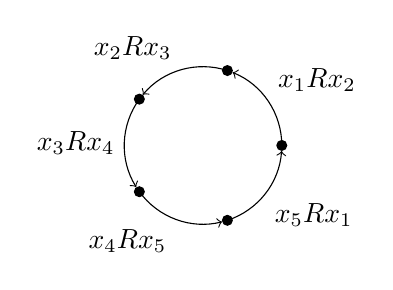
\begin{tikzpicture}
		\fill(1,0)circle(2pt)coordinate(A0);
		\fill({cos(72)},{sin(72)})circle(2pt)coordinate(A1);
		\fill({cos(144)},{sin(144)})circle(2pt)coordinate(A2);
		\fill({cos(216)},{sin(216)})circle(2pt)coordinate(A3);
		\fill({cos(288)},{sin(288)})circle(2pt)coordinate(A4);
		\begin{scope}[->]
			\draw(A0)arc[start angle=0,end angle=68,radius=1]node[midway,above right]{\(x_1 \rel{R} x_2\)};
			\draw(A1)arc[start angle=72,end angle=140,radius=1]node[midway,above left]{\(x_2 \rel{R} x_3\)};
			\draw(A2)arc[start angle=144,end angle=212,radius=1]node[midway,left]{\(x_3 \rel{R} x_4\)};
			\draw(A3)arc[start angle=216,end angle=284,radius=1]node[midway,below left]{\(x_4 \rel{R} x_5\)};
			\draw(A4)arc[start angle=288,end angle=356,radius=1]node[midway,below right]{\(x_5 \rel{R} x_1\)};
		\end{scope}
	\end{tikzpicture}
\end{center}
这是因为,如果我们有这样的环形成立,
那么根据传递性必有\(x_1 \rel{R} x_1\),
而这就与反自反性矛盾!

\begin{example}
设\(\rel{R}\)是\(A\)上的一个线性序,
证明:\(\rel{R}^{-1}\)也是\(A\)上的线性序.
\begin{proof}
由于\[
	\bigl( x \rel{R} y \land y \rel{R} z \implies x \rel{R} z \bigr)
	\iff
	\bigl( y \rel{R}^{-1} x \land z \rel{R}^{-1} y \implies z \rel{R}^{-1} x \bigr),
\]
可知\(\rel{R}^{-1}\)具有传递性.
又因为\(\rel{R}\)是\(A\)上的线性序,
所以对于\(\forall x,y \in A\),以下三个命题\[
	x \rel{R} y, \qquad
	x = y, \qquad
	y \rel{R} x
\]有且仅有一个成立;
换句话说,以下三个命题\[
	y \rel{R}^{-1} x, \qquad
	x = y, \qquad
	x \rel{R}^{-1} y
\]有且仅有一个成立;
可知\(\rel{R}^{-1}\)服从三一律.
综上所述,\(\rel{R}^{-1}\)也是\(A\)上的线性序.
\end{proof}
\end{example}

\subsection{偏序关系}
\begin{definition}
设\(\rel{R}\)是集合\(A\)上的二元关系,即\(\rel{R} \subseteq A^2\).
对于\(\forall x,y \in A\),若\[
	x\rel{R}y \land y\rel{R}x \implies x = y,
\]
则称“关系\(\rel{R}\)具有\DefineConcept{反对称性}(antisymmetric)”.
\end{definition}

\begin{definition}
设\(\rel{R}\)是集合\(A\)上的二元关系,即\(\rel{R} \subseteq A^2\).
如果\(\rel{R}\)同时具有自反性、反对称性、传递性,
则称“\(\rel{R}\)是\(A\)上的\DefineConcept{偏序关系}(ordering relation)”.
\end{definition}

\section{自然数}
一般而言,我们有两种途径,可以引入新的数学研究对象:公理法和构造法.
我们已经利用公理法引入了集合的概念.
集合是我们基于数学直觉和日常生活的原始认知之一.
在处理集合时,我们初步建立了一系列的公理%
(包括外延公理、对集公理、并集公理、幂集公理、子集公理、选择公理等).

在本节,我们要尝试引入自然数系统.
皮亚诺曾经在1889年给出过自然数的公理化定义.
但是我们不采纳公理法,转而采用构造法,
即基于集合的概念,定义自然数的概念,
通过对自然数的必要的性质的证明,取代皮亚诺公理体系.

\subsection{归纳集}
尽管自然数乍看之下不像是集合,
但是我们还是可以构造特定的集合,把它们定义为数字.
自然数的定义方式多种多样.
在1908年,策梅洛提议用\[
	\emptyset, \qquad
	\Set{\emptyset}, \qquad
	\Set{\Set{\emptyset}}, \qquad
	\Set{\Set{\Set{\emptyset}}}, \qquad
	\dotsc
\]代表自然数.
不久以后,冯·诺依曼提出了一种新的构造方式,
由于其优点,它成为了用集合定义自然数的标准构造.
冯诺依曼的构造方式的首要原则是把每个自然数看作所有“比它小的自然数”组成的集合.
我们可以把前四个自然数定义如下:\begin{align*}
	&0 \defeq \emptyset, \\
	&1 \defeq \Powerset0 = \Set{0} = \NaturalSet{1}, \\
	&2 \defeq \Powerset1 = \Set{0,1} = \NaturalSet{2}, \\
	&3 \defeq \Powerset2 = \Set{0,1,2} = \NaturalSet{3}.
\end{align*}
我们可以继续照此方式定义任意多个自然数.
可以注意到,在集合\(3=\Set{0,1,2}\)中有三个元素\(0,1,2\).
如果说\(A_3\)表示由所有“具有三个元素的集合”组成的类,
那么我们可以说集合\(3\)是\(A_3\)的代表.

容易发现,这些表示自然数的集合具有以下两个奇妙的性质:\[
	0 \in 1 \in 2 \in 3 \in \dotsb,
\]
以及\[
	0 \subseteq 1 \subseteq 2 \subseteq 3 \subseteq \dotsb.
\]

尽管我们已经给出了前四个自然数的定义,
也摸索出了定义任意自然数的大致思路,
但是我们还没有给出自然数的一般性定义.
也就是说,我们还没有定义由全部自然数组成的集合.
对于自然数集的确切定义是不能依赖类似由三个点表示的省略号或诸如“以此类推”这样的短语.
因此,我们首先需要给出一些基本概念的定义.
\begin{definition}[后继]\label{definition:集合论.后继的定义}
对于任意集合\(a\),把集合\[
	a \cup \Set{a}
\]
称为“\(a\)的\DefineConcept{后继}(successor)”,记为\(a^+\).
\end{definition}

利用后继符号,我们就可以将之前构造的用来表示自然数的集合重写为\[
	0=\emptyset, \qquad
	1=\emptyset^+, \qquad
	2=\emptyset^{++}, \qquad
	3=\emptyset^{+++}, \qquad
	\dotsc
\]
可以证明这些集合互不相等,例如\(\emptyset^+\neq\emptyset^{+++}\).

\begin{definition}[归纳集]\label{definition:集合论.归纳集的定义}
如果集合\(A\)满足
\begin{itemize}
	\item 空集是\(A\)的元素,即\[
		\emptyset \in A,
	\]
	\item 且\(A\)对后继封闭,即\[
		\forall a \in A : a^+ \in A,
	\]
\end{itemize}
则称“集合\(A\)是\DefineConcept{归纳的}(inductive)”,
或“集合\(A\)是\DefineConcept{归纳集}(inductive set)”.
\end{definition}
尽管我们还没有给出“无穷”或“无限”的正式定义,
但是我们还是可以凭借数学直觉非正式地看出任意归纳集都是无限无尽的.

利用列举法,我们可以将归纳集\(A\)表示为如下的一般形式:\[
	A = \Set{
		\emptyset, \emptyset^+, \emptyset^{++}, \dotsc,
		a, a^+, a^{++}, \dotsc,
		b, b^+, b^{++}, \dotsc
	}.
\]

\subsection{无穷公理}
尽管“归纳集”的概念在形式上有了清晰的定义,
我们可以照此方法尝试构造无穷多个不同的集合,
但是由于我们尚未建立确保“无穷集”存在的公理,
我们就无法证明存在这样一个“拥有无穷多个元素的集合”,
因此我们也就不能证明任何“归纳集”真实存在.
于是我们要用“无穷公理”补上这个漏洞.
\begin{axiom}[无穷公理]
总存在一个集合\(A\)是归纳集,即\[
	\exists A \bigl(
		\emptyset \in A
		\land
		\forall a \in A : a^+ \in A
	\bigr).
\]
\end{axiom}
无穷公理在英语中称作Infinity Axiom.

\subsection{自然数}
在无穷公理的加持下,我们终于可以定义自然数的概念了.
\begin{definition}\label{definition:集合论.自然数的定义}
如果集合\(a\)属于任意一个归纳集,那么称其为\DefineConcept{自然数}(natural number).
\end{definition}

下面我们证明“所有自然数的收集”构成一个集合.
\begin{theorem}\label{theorem:集合论.自然数集存在定理}
%@see: 《Elements of Set Theory》 P68. Theorem 4A
存在这样一个集合:它的元素都是自然数,任一自然数都是它的元素.
\begin{proof}
设\(A\)是一个归纳集(根据无穷公理,总可找到这样的\(A\)).
根据子集公理,%
\[
	\exists w,
	\forall x
	\left(
		\begin{array}{rcl}
			x \in w
			&\iff& x \in A \land x\ \text{属于所有异于\(A\)的其他归纳集} \\
			&\iff& x\ \text{属于所有归纳集}
		\end{array}
	\right).
\]
于是集合\(w\)的所有元素都是自然数,
所有的自然数都是集合\(w\)的元素.
\end{proof}
\end{theorem}
可以注意到,这个证明与\cref{theorem:集合论.系的交的唯一存在性} 的证明本质上相同.

这里我们用小写希腊字母\(\omega\)表记所有自然数的集合.
从\cref{theorem:集合论.自然数集存在定理} 的证明过程可以看出:
“\(x\)属于自然数集\(\omega\)”成立,
当且仅当“\(x\)是一个自然数”成立,
当且仅当“\(x\)属于每一个归纳集”成立.

利用描述法可以将自然数集定义为:
\[
	\omega
	\defeq
	\bigcap\Set{ A \given A\ \text{是归纳集} }.
\]
特别注意到:全部归纳集构成的类不是一个集合!

\begin{theorem}
%@see: 《Elements of Set Theory》 P69. Theorem 4B
自然数集\(\omega\)是归纳集,且它是任意一个归纳集的子集.
\begin{proof}
设\(A\)是任意的一个归纳集.

首先,由\hyperref[definition:集合论.归纳集的定义]{归纳集的定义}可知\(\emptyset \in A\),
于是\(\emptyset \in \omega\).

其次,对于任意集合\(a\),\(a \in \omega
\implies a \in A
\implies a^+ \in A
\implies a^+ \in \omega\).

因此\(\omega\)是归纳集,且\(\omega\)是任意一个归纳集的子集.
\end{proof}
\end{theorem}

既然\(\omega\)是归纳的,
那么根据归纳集的定义可知,\(0(=\emptyset)\)是自然数集的元素.
因此\(1(=0^+)\)在自然数集中,同理\(2(=1^+)\)和\(3(=2^+)\)也都在自然数集中.
于是我们说\(0,1,2,3\)都是自然数.
非必要的数学对象(即不是自然数的集合)都不在\(\omega\)中,
我们可以说:自然数集是“最小的”归纳集.
这句话可以更严谨地表述为下述“归纳原理”.
\begin{theorem}[归纳原理]
自然数集\(\omega\)的任意\DefineConcept{归纳子集}({\rm inductive subset})总是它自己.
\end{theorem}

这就引出“数学归纳法”的方法论,即:
如果我们要证明形如“对于每个自然数\(n\),涉及\(n\)的命题公式\(\lambda(n)\)成立”的命题,
我们可以基于自然数集\(\omega\),构造一个集合\[
	T = \Set{ n \in \omega \given \lambda(n) }.
\]
我们只要证明集合\(T\)是归纳的,
就能证明命题“对于每个自然数\(n\),涉及\(n\)的命题公式\(\lambda(n)\)成立”.

我们可以马上利用数学归纳法证明下面这个定理:
\begin{theorem}
%@see: 《Elements of Set Theory》 P69. Theorem 4C
除了\(0\)以外,所有自然数都是某个自然数的后继.
\begin{proof}
令集合\[
	T = \Set*{ n \in \omega \given n = 0 \lor \exists p \in \omega \bigl( n = p^+ \bigr) },
\]
则\(0 \in T\),且\(k \in T \implies k^+ \in T\).
因此根据归纳原则可知\(T = \omega\).
\end{proof}
\end{theorem}

\subsection{与皮亚诺公理的比较}
%TODO

\subsection{传递集}
\begin{definition}\label{definition:集合论.传递集的定义}
如果集合\(A\)的任一元素的每个元素都是\(A\)的元素,
那么称“集合\(A\)是\DefineConcept{传递的}(transitive)”,
或称“集合\(A\)是一个\DefineConcept{传递集}(transitive set)”,
即\begin{equation}\label{equation:集合论.传递集的定义式1}
	A\ \text{是传递集}
	\iff
	\forall x, \forall a \bigl(
		x \in a \in A
		\implies
		x \in A
	\bigr).
\end{equation}
\end{definition}
传递集\(A\)也可等价地定义为以下三种形式:
\begin{align}
	A\ \text{是传递集}
	&\iff
	\bigcup A \subseteq A;
	\label{equation:集合论.传递集的定义式2} \\
	&\iff
	a \in A \implies a \subseteq A;
	\label{equation:集合论.传递集的定义式3} \\
	&\iff
	A \subseteq \Powerset A.
	\label{equation:集合论.传递集的定义式4}
\end{align}

这里我们要注意区分“关系的传递性”与“传递集”这两个概念,它们是根本不同的!

\begin{example}
证明:空集\(\emptyset\)是传递集.
\begin{proof}
假设空集不是传递集,那么根据传递集的定义可知,\[
	\exists a, \exists x
	\bigl(
		x \in a \in \emptyset,
		x \notin \emptyset
	\bigr).
\]
但是根据空集公理,空集中根本就不存在满足条件的\(a\),矛盾!因此空集是传递集.
\end{proof}
\end{example}

\begin{example}
\def\a{\Set{\emptyset}}%
\def\b{\Set{\a}}%
\def\A{\Set{ \emptyset, \b }}%
集合\(\A\)不是一个传递集,%
这是因为\[
	\a \in \b \in \A,
	\quad\text{且}\quad
	\a \notin \A.
\]
\end{example}

\begin{example}
\(\Set{0,1,5}\)也不是传递集,
这是因为\[
	4 \in 5 \in \Set{0,1,5},
	\quad\text{且}\quad
	4 \notin \Set{0,1,5}.
\]
\end{example}

\begin{example}
%@see: 《Elements of Set Theory》 P73. Exercise 2.
证明:如果\(a\)是传递集,那么\(a^+\)也是传递集.
\begin{proof}
根据后继的定义,\(a^+ = a \cup \{a\}\),
那么总有\(a \in a^+ \lor a \subseteq a^+\),即\[
	\forall x
	\bigl(
		x \in a^+
		\implies
		x = a \lor x \in a
	\bigr)
\]恒成立.

当\(x = a\)时,
对于\(\forall t \in x\),
因为\(x = a \subseteq a^+\),
所以\(t \in a^+\).

当\(x \in a\)时,
因为\[
	a\ \text{是传递集}
	\iff
	\forall t
	\bigl(
		t \in x \in a
		\implies
		t \in a
	\bigr);
\]
又因为\(a \subseteq a^+\),
所以\(t \in a \subseteq a^+
\implies
t \in a^+\).

综上所述,\[
	\forall t, \forall x
	\bigl(
		t \in x \in a^+
		\implies
			t \in x = a
			\lor
			t \in x \in a
		\implies
		t \in a^+
	\bigr),
\]
\(a^+\)也是传递集.
\end{proof}
\end{example}

\begin{example}
%@see: 《Elements of Set Theory》 P73. Exercise 3.
证明:“\(a\)是传递集”的充要条件是“\(\Powerset a\)是传递集”.
\begin{proof}
先证充分性,假设\(\Powerset a\)是传递集.
根据幂集公理,恒有\[
	\forall x \bigl(
		x \in \Powerset a \iff x \subseteq a
	\bigr)
	\eqno(1)
\]成立;
又因为\(\Powerset a\)是传递集,
由\cref{equation:集合论.传递集的定义式2,equation:集合论.集的幂集的并等于集} 可知
\[
	a = \bigcup \Powerset a \subseteq \Powerset a;
	\eqno(2)
\]
于是\[
	\forall t, \forall x
	\bigl(
		t \in x \in a
		\overset{\text{(2)}}{\implies}
		t \in x \in \Powerset a
		\overset{\text{(1)}}{\implies}
		t \in x \subseteq a
		\implies
		t \in a
	\bigr),
\]
因此\(a\)是传递集.

再证必要性,假设\(a\)是传递集.
由\cref{equation:集合论.传递集的定义式4} 可知
\[
	a \subseteq \Powerset a;
	\eqno(3)
\]
于是\[
	\forall t, \forall y \bigl(
		t \in y \in \Powerset a
		\overset{\text{(1)}}{\implies}
		t \in y \subseteq a
		\implies
		t \in a
		\overset{\text{(3)}}{\implies}
		t \in \Powerset a
	\bigr);
\]
因此\(\Powerset a\)也是传递集.
\end{proof}
\end{example}

\begin{example}
%@see: 《Elements of Set Theory》 P73. Exercise 4.
证明:如果\(A\)是传递集,那么\(\bigcup A\)也是传递集.
\begin{proof}
因为\(A\)是传递集,由\cref{equation:集合论.传递集的定义式2} 可知
\[
	\bigcup A \subseteq A;
\]
又由\cref{equation:集合论.系的并的幂集包含系} 可知\[
	A \subseteq \Powerset \bigcup A;
\]
所以\[
	\bigcup A \subseteq \Powerset \bigcup A,
\]
由\cref{equation:集合论.传递集的定义式4} 可知\(\bigcup A\)是传递集.
\end{proof}
\end{example}

\begin{theorem}
%@see: 《Elements of Set Theory》 P72. Theorem 4E
如果\(a\)是传递集,那么\(\bigcup\left( a^+ \right) = a\).
\begin{proof}
直接计算得\begin{align*}
	\bigcup\left( a^+ \right)
	&= \bigcup (a \cup \{a\}) \\
	&= \bigcup a \cup \bigcup\Set{a} \\
	&= \bigcup a \cup a \\
	&= a.
	\qedhere
\end{align*}
\end{proof}
\end{theorem}

\begin{example}
%@see: 《Elements of Set Theory》 P73. Exercise 6.
证明:如果\(\bigcup\left( a^+ \right) = a\),那么\(a\)是传递集.
%TODO
\end{example}

\begin{example}
%@see: 《Elements of Set Theory》 P73. Exercise 5.
设\(\mathscr{A}\)中的每一个元素都是传递集.
证明:\begin{enumerate}
	\item \(\bigcup \mathscr{A}\)是传递集.
	\item 当\(\mathscr{A}\)非空时,\(\bigcap \mathscr{A}\)是传递集.
\end{enumerate}
%TODO
\end{example}

\begin{theorem}
%@see: 《Elements of Set Theory》 P72. Theorem 4F
任一自然数都是传递集.
\begin{proof}
用数学归纳法证明.
首先,\(\emptyset\)是传递集.
假设自然数\(k\)也是传递集,那么\[
	\bigcup k^+ = k \subseteq k^+,
\]
又因为\(k^+\)也是传递集,
所以每个自然数都是传递集.
\end{proof}
\end{theorem}

\begin{theorem}
%@see: 《Elements of Set Theory》 P72. Theorem 4G
自然数集\(\omega\)是传递集.
\begin{proof}
用数学归纳法证明.
欲证\(\forall a \in \omega \bigl(
	a \subseteq \omega
\bigr)\),
只需证集合\[
	T = \Set{n \in \omega \given n \subseteq \omega}
\]是传递的.
显然\(\emptyset \in T\).
假设\(k \in T\),那么有\[
	k \subseteq \omega
	\land
	\{k\} \subseteq \omega;
\]
同时\(k \cup \{k\} \subseteq \omega\),从而\(k^+ \in T\).
因此\(T\)是传递的,而自然数集\(\omega\)是传递集.
\end{proof}
\end{theorem}
上述定理也可表述为:
每个自然数都是由自然数组成的集合.
以后我们还可以将这个定理加强为:
每个自然数都是由比它小的自然数组成的集合.

\subsection{自然数的递归}
考虑一个映射\(h\colon \omega \to A\),
我们只知道\(h(0)\)的取值,
以及映射\(F\colon A \to A\)满足\[
	h(n^+) = F(h(n))
	\quad(n\in\omega).
\]
由此,虽然我们不知道映射\(h\)的具体表达式,
但我们总能依次计算出\(h(n)\ (n\in\omega)\)的取值:\[
	h(0), \qquad
	h(1) = F(h(0)), \qquad
	h(2) = F(h(1)), \qquad
	\dotsc
\]

接下来,考虑任给一个集合\(A\),再从中任取一个元素\(a\),
以及给定一个映射\(F\colon A \to A\).
那么我们要怎么证明存在一个映射\(h\colon \omega \to A\),
使得\(h(0) = a\),且对\(\forall n\in\omega\)总有\[
	h(n^+) = F(h(n)).
\]
在前一段,我们学会了怎么计算映射\(h\)(前提是这样的映射\(h\)存在).
现在我们想要证明存在一个映射\(h\)满足上述条件.

\begin{theorem}\label{theorem:集合论.递归定理}
%@see: 《Elements of Set Theory》 P73. Recursion Theorem on omega
设\(A\)是集合,\(a \in A\),映射\(F\colon A \to A\),
那么存在一个唯一的映射\(h\colon \omega \to A\),使得\[
	h(0) = a; \qquad
	h(n^+) = F(h(n)), \quad n\in\omega.
\]
\begin{proof}
为了方便后续证明,我们首先在这里提出一个概念:
称“映射\(v\)是\emph{容许的}(acceptable)”,
当且仅当以下三个条件同时成立:
\begin{enumerate}[label={(\roman*)}]
	\item\label{item:集合论.容许映射条件1}
	\(\dom v \subseteq \omega\)且\(\ran v \subseteq A\);

	\item\label{item:集合论.容许映射条件2}
	\(0 \in \dom v
	\implies
	v(0) = a\);

	\item\label{item:集合论.容许映射条件3}
	对任意\(n \in \omega\),总有\(n^+ \in \dom v
	\implies
	n \in \dom v \land v(n^+) = F(v(n))\).
\end{enumerate}
令\(\mathscr{K}\)为所有容许映射的汇集,
再令\(h = \bigcup \mathscr{K}\),
那么有\begin{equation}
	\begin{split}
		\opair{n,y} \in h
		&\iff
		\opair{n,y}\ \text{是某个容许映射\(v\)的元素} \\
		&\iff
		\text{对某个容许映射\(v\),总有\(v(n) = y\)成立}.
	\end{split}
	\tag1
\end{equation}
我们要证明\(h\)符合定理的要求,可以将证明细分为四个部分,
即证明\(h\)是一个映射,且它是容许的,
它的定义域是整个自然数集,以及这个映射是唯一的:
\begin{enumerate}
	\item 我们首先证明\(h\)是映射.
	%Proving this will, in effect, amount to showing that two acceptable functions
	%always agree with each other whenever both are defined.
	%TODO 这句不知道怎么翻译好呢
	令\[
		S = \Set{ n \in \omega
		\given
		\text{至多只有一个}\ y\ \text{满足}\ \opair{n,y} \in h }.
	\]
	我们需要证明\(S\)是归纳集.

	如果\[
		\opair{0,y_1} \in h
		\quad\text{且}\quad
		\opair{0,y_2} \in h,
	\]
	那么根据(1)式,存在容许映射\(v_1,v_2\),使得\[
		v_1(0) = y_1
		\quad\text{且}\quad
		v_2(0) = y_2;
	\]
	再根据\hyperref[item:集合论.容许映射条件2]{容许映射条件(ii)} 可知\(y_1 = a = y_2\),
	因此\(0 \in S\).

	假设\(k \in S\),
	欲证\(k^+ \in S\).
	朝着这个方向,我们又假设\[
		\opair{k^+,y_1} \in h
		\quad\text{且}\quad
		\opair{k^+,y_2} \in h.
	\]
	同样地,必定存在容许映射\(v_1,v_2\),使得\[
		v_1(k^+) = y_1
		\quad\text{且}\quad
		v_2(k^+) = y_2.
	\]
	再根据\hyperref[item:集合论.容许映射条件3]{容许映射条件(iii)} 可知\[
		y_1 = v_1(k^+) = F(v_1(k))
		\quad\text{且}\quad
		y_2 = v_2(k^+) = F(v_2(k)).
	\]
	又因为\(k \in S\),
	我们有\(\opair{k,v_1(k)},\opair{k,v_2(k)} \in h\),
	从而有\(v_1(k) = v_2(k)\),
	因此\[
		y_1 = F(v_1(k)) = F(v_2(k)) = y_2,
	\]
	这就说明\(k^+ \in S\).

	于是,\(S\)是归纳集,而且它恰好就是自然数集\(\omega\),
	从而\(h\)是一个映射.

	\item 现在我们来证明\(h\)是容许的.
	既然我们已经证明\(h\)是映射,
	那么根据(1)式,
	显然有\(\dom h \subseteq \omega\)且\(\ran h \subseteq A\).

	我们先来检验\hyperref[item:集合论.容许映射条件2]{容许映射条件(ii)}.
	如果\(0 \in \dom h\),
	那么必定存在某个容许映射\(v\)满足\(v(0) = h(0)\).
	既然\(v(0) = a\),我们就有\(h(0) = a\).

	我们再来检验\hyperref[item:集合论.容许映射条件3]{容许映射条件(iii)}.
	假设\(n^+ \in \dom h\).
	同样地,必定存在某个容许映射\(v\)满足\(v(n^+) = h(n^+)\).
	既然\(v\)是容许的,我们就有\(n \in \dom v\),\(v(n) = h(n)\),以及\[
		h(n^+) = F(h(n)) = F(v(n)) = v(n^+).
	\]

	于是,\(h\)是容许的.

	\item 现在我们来证明\(h\)的定义域是整个自然数集,
	即\(\dom h = \omega\).
	实际上我们只需证\(\dom h\)是归纳集.
	由于映射\(\Set{\opair{0,a}}\)是容许的,
	所以\(0 \in \dom h\).
	假设\(k \in \dom h\),只需证\(k^+ \in \dom h\).
	如果这条路走不通,那么考虑\[
		v = h \cup \Set{\opair{k^+,F(h(k))}}.
	\]
	易见\(v\)是一个映射,且\(\dom v \subseteq \omega\),\(\ran v \subseteq A\).
	因此只需证\(v\)是容许的.

	由于\(v(0) = h(0) = a\),
	\hyperref[item:集合论.容许映射条件2]{容许映射条件(ii)} 成立.
	对于\hyperref[item:集合论.容许映射条件3]{容许映射条件(iii)},
	可以分为两种情形.
	如果\(n^+ \in \dom v\ (n^+ \neq k^+)\),
	那么\(n^+ \in \dom h\)且\(v(n^+) = h(n^+) = F(h(n)) = F(v(n))\).
	其他情形当\(n^+ = k^+\)时出现.
	既然后继是一一映射,那么\(n=k\).
	根据假设\(k \in \dom h\).
	因此\[
		v(k^+) = F(h(k)) = F(v(k))
	\]
	且\hyperref[item:集合论.容许映射条件3]{容许映射条件(iii)} 成立.
	可见,\(v\)是容许的.
	但是,接下来我们有\(v \subseteq h\),
	从而\(k^+ \in \dom h\).

	于是,\(\dom h\)是归纳集,且\(\dom h = \omega\).

	\item 最后我们证明\(h\)是唯一的.
	假设映射\(h_1,h_2\)都符合定理的要求.
	令\[
		S = \Set{ n \in \omega \given h_1(n) = h_2(n) }.
	\]
	易见\(S\)是归纳集.
	%TODO 证明“\(S\)是归纳集”的步骤参考本节 Exercise 7

	于是,\(S = \omega\)且\(h_1 = h_2\).
\end{enumerate}
\end{proof}
\end{theorem}
我们把\cref{theorem:集合论.递归定理} 称为\DefineConcept{递归定理}.

\subsection{自然数的算术运算}
我们可以利用\hyperref[theorem:集合论.递归定理]{递归定理}定义自然数集上的加法和乘法.

\begin{definition}
%@see: 《Elements of Set Theory》 P79. Definition
任给一个映射\(f\colon A^2 \to A\),
我们称“\(f\)是定义在集合\(A\)上的一个%
\DefineConcept{二元代数运算}(binary arithmetic operation)”.
\end{definition}

我们首先尝试构造自然数的加法.

任取\(m \in \omega\),
根据\hyperref[theorem:集合论.递归定理]{递归定理}%
易证存在唯一映射\(A_m\colon \omega \to \omega\)满足\[
	A_m(0) = m; \qquad
	A_m(n^+) = (A_m(n))^+, \quad n \in \omega.
\]
\begin{definition}
%@see: 《Elements of Set Theory》 P79. Definition
\DefineConcept{加法}(addition,用符号“\(+\)”表记)%
是定义在自然数集\(\omega\)上的一个二元代数运算,
它满足:对于任意自然数\(m,n\),总有\[
	m + n = A_m(n).
\]
\end{definition}
我们可以把加法运算写成关系的形式:\[
	+ \defeq \Set{
		\opair{\opair{m,n},p}
		\given
		m \in \omega
		\land
		n \in \omega
		\land
		p = A_m(n)
	}.
\]

\begin{theorem}
%@see: 《Elements of Set Theory》 P79. Theorem 4I
对于任意自然数\(m,n\),总有\begin{gather}
	m + 0 = m, \\
	m + n^+ = (m+n)^+.
\end{gather}
\end{theorem}

接下来我们构造自然数的乘法.

类似于加法的构造,任取\(m \in \omega\),
易证存在唯一映射\(M_m\colon \omega \to \omega\)满足\[
	M_m(0) = 0; \qquad
	M_m(n^+) = M_m(n) + m, \quad n \in \omega.
\]
\begin{definition}
乘法(multiplication,用符号“\(\times\)”或“\(\cdot\)”表记)%
是定义在自然数集\(\omega\)上的一个二元代数运算,
它满足:对于任意自然数\(m,n\),总有\[
	m \times n = M_m(n).
\]
\end{definition}
我们可以把乘法运算写成关系的形式:\[
	\times \defeq \Set{
		\opair{\opair{m,n},p}
		\given
		m \in \omega
		\land
		n \in \omega
		\land
		p = M_m(n)
	}.
\]

\begin{theorem}
%@see: 《Elements of Set Theory》 P79. Theorem 4J
对于任意自然数\(m,n\),总有\begin{gather}
	m \cdot 0 = 0, \\
	m \cdot n^+ = m \cdot n + m.
\end{gather}
\end{theorem}

我们在定义加法和乘法以后,
还可以类似地定义自然数的\DefineConcept{乘幂}(exponentiation),
并且可以给出:对于任意自然数\(m,n\),总有\begin{gather}
	m^0 = 1, \quad m \neq 0; \\
	m^{(n^+)} = m^n \cdot m.
\end{gather}

\begin{theorem}
%@see: 《Elements of Set Theory》 P79. Theorem 4K
对于任意自然数\(m,n,p\),以下命题恒成立:
\begin{enumerate}
	\item 加法结合律(associative law for addition)\[
		m+(n+p)=(m+n)+p.
	\]
	\item 加法交换律(commutative law for addition)\[
		m+n=n+m.
	\]
	\item 乘法分配律(distributive law)\[
		m \cdot (n+p) = m \cdot n + m \cdot p.
	\]
	\item 乘法结合律(associative law for multiplication)\[
		m \cdot (n \cdot p) = (m \cdot n) \cdot p.
	\]
	\item 乘法交换律(commutative law for multiplication)\[
		m \cdot n = n \cdot m.
	\]
\end{enumerate}
\end{theorem}
这些命题依靠数学归纳法可以轻松得证,故略去证明.

\subsection{自然数的序}
%TODO

\section{实数}
%TODO

\section{集合的大小}
\begin{definition}
一个集合所包含的元素的个数,称作集合的\DefineConcept{基数}(cardinal)、\DefineConcept{元数}或\DefineConcept{浓度},记作\(\card(A)\)或\(\abs{A}\).
\end{definition}

\begin{definition}
只含有限个元素的集合称为\DefineConcept{有限集}(finite set).
不是有限集的集合称为\DefineConcept{无限集}(infinite set).
\end{definition}

\begin{property}
有限集\(A\)对应的幂集的大小为\[
	\abs{\Powerset A} = 2^{\abs{A}}.
\]
%TODO
%\begin{proof}
%\end{proof}
\end{property}

\begin{example}
设\(A\)、\(B\)是任意两个集合,试证:
\(\abs{A \cup B} + \abs{A \cap B} = \abs{A} + \abs{B}\).
%TODO
\end{example}

\section{数集}
\subsection{常见数集的总结}
\begin{center}
\begin{tabular}{c|l|l}
\hline
名称 & 记法 & 定义 \\ \hline
自然数集 & \(\mathbb{N}\) & \(\{ 0,1,2,3,\dotsc \}\) \\
正整数集 & \(\mathbb{N}^+\) & \(\{ 1,2,3,\dotsc \}\) \\
整数集 & \(\mathbb{Z}\) & \(\{ \dotsc,-2,-1,0,1,2,3,\dotsc \}\) \\
有理数集 & \(\mathbb{Q}\) & \(\{ \frac{p}{q} \mid p \in \mathbb{Z}, q \in \mathbb{N}^+, \text{p与q互质} \}\) \\
实数集 & \(\mathbb{R}\) \\
非零实数集 & \(\mathbb{R}^*\) & \(\{ x \in \mathbb{R} \mid x \neq 0 \}\) \\
正实数集 & \(\mathbb{R}^+\) & \(\{ x \in \mathbb{R} \mid x > 0 \}\) \\
扩展实数集 & \(\overline{\mathbb{R}}\) & \(\mathbb{R} \cup (-\infty,+\infty)\) \\
复数集 & \(\mathbb{C}\) & \(\{ z = x + \iu y \mid x,y \in \mathbb{R}; \iu^2 = -1 \}\) \\ \hline
\end{tabular}
\end{center}

\section{区间}
\begin{definition}
\DefineConcept{区间}(interval)是实数集的子集.
设\(a,b\in\mathbb{R}\),且\(a<b\).
定义:
\begin{center}
\begin{tabular}{|*4{c|}} \hline
	\multicolumn{2}{|c|}{名称} & 记法 & 描述法表示 \\ \hline
	\multicolumn{2}{|c|}{开区间(open interval)} & \((a,b)\) & \(\Set{ x \given a < x < b }\) \\ \hline
	\multicolumn{2}{|c|}{闭区间(closed interval)} & \([a,b]\) & \(\Set{ x \given a \leqslant x \leqslant b }\) \\ \hline
	\multirow{2}{*}{半开区间(half-closed interval)} & 左开右闭区间 & \((a,b]\) & \(\Set{ x \given a < x \leqslant b }\) \\ \cline{2-4}
	& 左闭右开区间 & \([a,b)\) & \(\Set{ x \given a \leqslant x < b }\) \\ \hline
\end{tabular}
\end{center}
其中,\(a\)、\(b\)称为区间的\DefineConcept{端点},
\(b-a\)称为区间的\DefineConcept{长度}.
像这样,端点\(a\)、\(b\)都是有限实数的区间称为\DefineConcept{有限区间}.

特别地,有如下的定义:
\[
	(a,+\infty) = \Set{ x \given x > a },
\]\[
	[a,+\infty) = \Set{ x \given x \geqslant a },
\]\[
	(-\infty,b) = \Set{ x \given x < b },
\]\[
	(-\infty,b] = \Set{ x \given x \leqslant b },
\]\[
	(-\infty,+\infty) = \Set{ x \given x \in \mathbb{R} }.
\]
像这样,端点中任一或全部为无穷大的,统称为\DefineConcept{无限区间}.
\end{definition}

\section{上确界与下确界}
\begin{definition}
设\(X\)是实数的有界子集.

如果\(\forall x \in X\)都有\(x \geqslant m\),%
且对于\(\forall \varepsilon > 0\)都\(\exists \alpha \in X\)使\(\alpha < m + \varepsilon\)成立,%
则数\(m\)称为集合\(X\)的\DefineConcept{下确界},记作\(\inf{x}\).

如果\(\forall x \in X\)都有\(x \leqslant M\),%
且对于\(\forall \varepsilon > 0\)都\(\exists \beta \in X\)使\(\beta > M - \varepsilon\)成立,%
则数\(M\)称为集合\(X\)的\DefineConcept{上确界},记作\(\sup{x}\).

如果集合\(X\)下方无界,则记\[
\inf{x} = -\infty;
\]如果集合\(X\)上方无界,则记\[
\sup{x} = +\infty.
\]
\end{definition}

\section{邻域}
\begin{definition}
在数域\(P\)上取一点\(a \in P^n\)(\(n\in\mathbb{N}^+\)),区域\[
\Set{b \in P^n \given \abs{b - a} < \delta}
\]称为点\(a\)的\(\delta\)\DefineConcept{邻域},记作\(U(a,\delta)\);其中,点\(a\)称为邻域的\DefineConcept{中心},\(\delta\)称为邻域的\DefineConcept{半径}.

特别地,区域\[
\Set{b \in P^n \given 0 < \abs{b - a} < \delta}
\]称为点\(a\)的\DefineConcept{去心\(\delta\)邻域},记作\(\mathring{U}(a,\delta)\).

在不需要强调邻域半径\(\delta\)的时候,邻域\(U(a,\delta)\)简记为\(U(a)\),去心邻域\(\mathring{U}(a,\delta)\)简记为\(\mathring{U}(a)\).

特别地,对于\(P^1\)上任意一点\(a\),把开区间\((a-\delta,a)\)称为\(a\)的\DefineConcept{左\(\delta\)邻域}(简称\DefineConcept{左邻域}),把开区间\((a,a+\delta)\)称为\(a\)的\DefineConcept{右\(\delta\)邻域}(简称\DefineConcept{右邻域}).
\end{definition}

\begin{property}
显然地,总有\(\mathring{U}(a,\delta) \subsetneqq U(a,\delta)\)成立.
\end{property}

\section{平面上的点与点集}
\subsection{平面上的点与点集的关系}
\begin{definition}
设点\(P\in\mathbb{R}^2\),点集\(S\subseteq\mathbb{R}^2\).
定义:\begin{enumerate}
\item 若\(\exists U(P)\)使得\[
U(P) \subseteq S,
\]则称点\(P\)为\(S\)的\DefineConcept{内点}(interior),记作\(P \in I(S)\).
(如\cref{figure:集合论.平面上的点与点集的关系} 中,\(P_1\)为\(S\)的内点);

\item 若\(\exists U(P)\)使得\[
U(P) \cap S = \emptyset,
\]则称点\(P\)为\(S\)的\DefineConcept{外点}(exterior),记作\(P \in E(S)\).
(如\cref{figure:集合论.平面上的点与点集的关系} 中,\(P_2\)为\(S\)的外点);

\item 若\(\forall U(P)\)都有\[
\exists a \bigl( a \in U(P) \land a \in S \bigr)
\quad\text{且}\quad
\exists b \bigl( b \in U(P) \land b \notin S \bigr),
\]则称点\(P\)为\(S\)的\DefineConcept{边界点},记作\(P \in \partial{S}\).
(如\cref{figure:集合论.平面上的点与点集的关系} 中,\(P_3\)为\(S\)的边界点);
\end{enumerate}

\begin{figure}[ht]
\centering
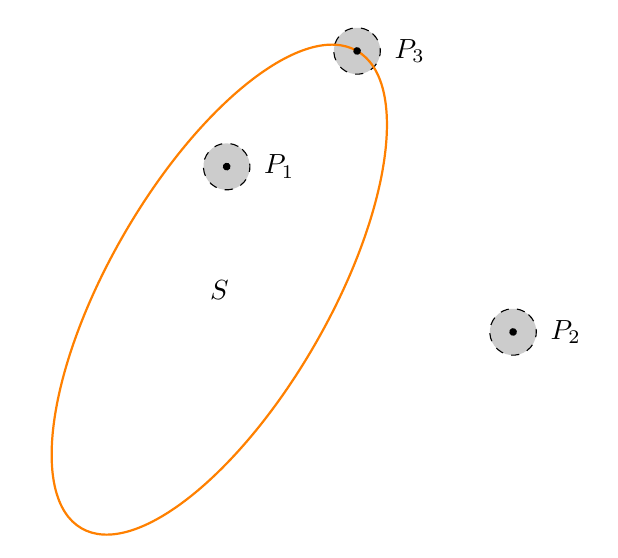
\begin{tikzpicture}[scale=.7]
\filldraw[rotate=60,draw=black,dashed,fill=gray!40]
	(2,1)circle(12pt)
	(2,-5)circle(12pt)
	(5,0)circle(12pt);
\draw[orange,rotate=60,thick](0,0)ellipse[x radius=5,y radius=2];
\draw (0,0)node{\(S\)};
\fill[rotate=60]
	(2,1)circle(2pt)node[right=10pt]{\(P_1\)}
	(2,-5)circle(2pt)node[right=10pt]{\(P_2\)}
	(5,0)circle(2pt)node[right=10pt]{\(P_3\)};
\end{tikzpicture}
\caption{平面上的点与点集的关系}
\label{figure:集合论.平面上的点与点集的关系}
\end{figure}
\end{definition}

\begin{property}
设点集\(S\subseteq\mathbb{R}^2\).
任意一点\(P\in\mathbb{R}^2\)要么是\(S\)的内点,要么是\(S\)的外点,要么是\(S\)的边界点.

换言之,任意点集\(S\)的内点、外点和边界点的集合均无交集,即:
\begin{enumerate}
\item \(I(S) \cap E(S) = \emptyset\).
\item \(\partial{S} \cap I(S) = \emptyset\).
\item \(\partial{S} \cap E(S) = \emptyset\).
\end{enumerate}
\end{property}

\begin{definition}
设点\(P\)和点集\(S\)满足\(P \in S\).
定义:若\(\exists \mathring{U}(P)\)使得\[
\mathring{U}(P) \cap S = \emptyset,
\]则称\(P\)为\(S\)的\DefineConcept{孤立点}(acnode),记作\(P \in A(S)\).
\end{definition}

\begin{property}
\(S\)的内点必属于\(S\),即\[
P \in I(S) \implies P \in S
\]或\[
I(S) \subseteq S.
\]
\begin{proof}
\[
\left. \begin{array}{r}
P \in I(S) \iff \exists U(P) :\: U(P) \subseteq S \\
P \in U(P)
\end{array} \right\}
\implies P \in S.
\qedhere
\]
\end{proof}
\end{property}

\begin{property}
\(S\)的外点必不属于\(S\),即\(P \in E(S) \implies P \notin S\).
\begin{proof}
\begin{align*}
\left. \begin{array}{r}
P \in E(S) \iff \exists U(P) :\: U(P) \cap S = \emptyset \\
P \in U(P) \iff \{P\} \subseteq U(P) \implies \{P\} \cap S \subseteq U(P) \cap S
\end{array} \right\}
\implies& \{P\} \cap S \subseteq \emptyset \\
\implies \{P\} \cap S = \emptyset
\implies P \notin S.&
\qedhere
\end{align*}
\end{proof}
\end{property}

\begin{example}
点集的边界点可能属于该点集,也可能不属于它.例如,实轴上的左闭右开区间\([a,b)\)有两个边界点\(a\)和\(b\),但\(a \in [a,b)\)而\(b \notin [a,b)\).
\end{example}

\begin{definition}
设点\(P\in\mathbb{R}^2\),点集\(S\subseteq\mathbb{R}^2\).
定义:如果点\(P\)的任意邻域内总有\(S\)中的无穷多个点,则称\(P\)是\(S\)的\DefineConcept{聚点}(cluster),记作\(P \in C(S)\),即\[
P \in C(S)
\iff
\forall\delta>0,\exists Q \in S : Q \in \mathring{U}(P,\delta).
\]称点集\(S\)的聚点的集合\(C(S)\)为\(S\)的\DefineConcept{导集}(derived set).
\end{definition}
任取点集\(S\)的一个聚点\(P_C\).由聚点的定义可知,\(P_C\)可以属于\(S\),也可以不属于\(S\).

\begin{theorem}
点\(P\)是点集\(S\)的聚点的充要条件是:在\(P\)的任意邻域内总有异于点\(P\)而属于\(S\)的一个点,即\[
\forall \delta>0 \bigl[
	\mathring{U}(P,\delta) \cap S \neq \emptyset
\bigr].
\]
\end{theorem}

\begin{property}
点集的内点均是其聚点,即\(I(S) \subseteq C(S)\).
\begin{proof}
由内点的定义有\(P \in I(S) \iff \exists \delta_1>0 :\: U(P,\delta_1) \subseteq S\).

当\(0 < \delta_2 \leqslant \delta_1\)时,有\[
\mathring{U}(P,\delta_2)
\subseteq U(P,\delta_1)
\subseteq S,
\]所以\[
\mathring{U}(P,\delta_2) \cap S
= \mathring{U}(P,\delta_2)
\neq \emptyset.
\]

当\(\delta_2 > \delta_1\)时,有\[
\emptyset \neq \mathring{U}(P,\delta_1) \subsetneqq U(P,\delta_1) \subseteq S,
\]\[
\mathring{U}(P,\delta_2) \cap S
\supseteq \mathring{U}(P,\delta_1) \cap S \neq \emptyset.
\]

综上所述,对于\(\forall \delta_2 > 0\)都有\(\mathring{U}(P,\delta_2) \cap S \neq \emptyset\)成立,即\(P \in C(S)\).
\end{proof}
\end{property}

\begin{property}
点集的外点不是其聚点,即\(P \in E(S) \implies P \notin C(S)\).
\begin{proof}
因为\(P \in E(S)\),所以\(\exists \delta > 0: U(P,\delta) \cap S = \emptyset\).又因为\(\mathring{U}(P,\delta) \subsetneqq U(P,\delta)\),所以\[
U(P,\delta) \cap S \supsetneqq \mathring{U}(P,\delta) \cap S = \emptyset,
\]从而有\(P \notin C(S)\).
\end{proof}
\end{property}

\begin{property}
点集的孤立点不是聚点,即\(P \in A(S) \implies P \notin C(S)\).
\begin{proof}
\(P \in A(S) \implies \exists \delta > 0 : \mathring{U}(P,\delta) \cap S = \emptyset \iff P \notin C(S)\).
\end{proof}
\end{property}

\begin{property}
点集的孤立点必不是其内点,点集的内点也必不是其孤立点,即\[
P \in A(S) \implies P \notin I(S),
\]\[
P \in I(S) \implies P \notin A(S).
\]
\end{property}

\begin{property}
点集的孤立点必不是其外点,点集的外点也必不是其孤立点,即\[
P \in A(S) \implies P \notin E(S),
\]\[
P \in E(S) \implies P \notin A(S).
\]
\end{property}

\begin{property}
点集的孤立点必是其边界点,即\(A(S) \subseteq \partial{S}\).
\end{property}

\begin{property}
点集的边界点可能是聚点,也可能不是聚点.
\end{property}

\begin{definition}
设点集\(S \subseteq \mathbb{R}^2\).

若\(S\)的点皆为它的内点,则称\(S\)为\DefineConcept{开集}.若\(S\)的所有边界点都属于\(S\)(即\(\partial S \subseteq S\)),或所有聚点皆属于\(S\)(即\(C(S) \subseteq S\)),则称\(S\)为\DefineConcept{闭集}.

若\(\exists r > 0\),使得\[
S \subseteq U(O,r),
\]其中\(O\)是坐标原点\(\opair{0,0}\),则称“\(S\)是\DefineConcept{有界的}”或“\(S\)是\DefineConcept{有界集}”;
否则称“\(S\)是\DefineConcept{无界的}”或“\(S\)是\DefineConcept{无界集}”.

若\(S\)中任意两点均可用一条全含于\(S\)内的折线相连接,则称“\(S\)是\DefineConcept{连通的}”或“\(S\)是\DefineConcept{连通集}”.

若\(S\)既是连通集又是开集,则称\(S\)为\DefineConcept{开区域}.
开区域\(S\)及其边界\(\partial S\)的并集\(S + \partial S\)称为\DefineConcept{闭区域}%
(简称\DefineConcept{闭域},常记作\(\overline{S}\)).
开区域与闭区域统称\DefineConcept{区域}.
\end{definition}

\begin{definition}\label{definition:集合论.平面区域的连通性}
%@see: https://mathworld.wolfram.com/SimplyConnected.html
%@see: https://mathworld.wolfram.com/MultiplyConnected.html
如果在平面区域\(S \subseteq \mathbb{R}^2\)内,%
任一闭曲线所围的部分都属于\(S\),%
则称“平面区域\(S\)是\DefineConcept{单连通的}(simply-connected)”;
否则称“平面区域\(S\)是\DefineConcept{复连通的}(multiply-connected)”.
\end{definition}
